\documentclass[conference]{IEEEtran}
\IEEEoverridecommandlockouts

\usepackage{cite}
\usepackage{amsmath,amssymb,amsfonts}
\usepackage{textcomp}
\usepackage{xcolor}
\usepackage{graphicx}
\usepackage[caption=false,font=footnotesize]{subfig}
\usepackage{booktabs}

% figures/ on Overleaf; ../figures/ when compiled inside the code repository
\graphicspath{{figures/}{../figures/}}

\newcommand{\todo}[1]{\textcolor{red}{[TODO: #1]}}
\newcommand{\Ein}{E_{\mathrm{in}}}
\newcommand{\Eout}{E_{\mathrm{out}}}
\newcommand{\Eaug}{E_{\mathrm{aug}}}
\newcommand{\wlin}{\mathbf{w}_{\mathrm{lin}}}
\newcommand{\w}{\mathbf{w}}
\newcommand{\x}{\mathbf{x}}
\newcommand{\X}{\mathrm{X}}
\newcommand{\Z}{\mathrm{Z}}
\newcommand{\y}{\mathbf{y}}
\newcommand{\T}{^{\mathsf T}}

\begin{document}

\title{Learning, Overfitting, and Regularization\\with Linear Models from Scratch}

\author{\IEEEauthorblockN{1\textsuperscript{st} Dauletkali Toktybayev}
\IEEEauthorblockA{\textit{School of Computing and Artificial Intelligence} \\
\textit{Nazarbayev University}\\
Astana, Kazakhstan \\
dauletkali.toktybayev@nu.edu.kz}
\and
\IEEEauthorblockN{2\textsuperscript{nd} Nuradil Serik}
\IEEEauthorblockA{\textit{School of Computing and Artificial Intelligence} \\
\textit{Nazarbayev University}\\
Astana, Kazakhstan \\
nuradil.serik@nu.edu.kz}}

\maketitle

\begin{abstract}
We implement the pocket perceptron with the linear regression and logistic regression, both with weight decay and lasso regularization, using NumPy. They are employed to test learning theory using the known target, noise and out-of-sample error on a simulated dataset and then determine if they apply to real data. On simulated data we can check the theory exactly. The in-sample error of the least squares is equal to its formula, whereas the error of the textbook out-of-sample approximation is incorrect for small sample sizes, as the number of parameters approaches the sample size. The condition number is squared when formulating the normal equations. Overfitting heatmaps distinguish between stochastic and deterministic noise. Closed-form leave-one-out validation agrees with brute-force refitting to twelve digits, and picking features on all the data makes pure noise seem a ninety percent chance of being predictable. Add censored targets (California housing), separated classes and weak hand-crafted features (breast cancer, handwritten digits). Regularization reduces the cross-validated error of linear regression on raw pixels by nearly a factor of three for the capstone, but makes no difference for a two-feature model whose error is bias.
\end{abstract}

\begin{IEEEkeywords}
perceptron, linear regression, logistic regression, regularization, cross-validation, overfitting
\end{IEEEkeywords}

%==============================================================
\section{Introduction}
For linear models, most statements about generalization have exact forms that a simulation can check. On simulated data we know the target $f$, the noise and the true $\Eout$, so we compare each formula with a simulation directly.

We write every algorithm, metric and validation routine in NumPy, with \texttt{scipy.linalg}, \texttt{scipy.optimize} and \texttt{scipy.special} where the brief allows them. We use scikit-learn only to load data and in cells marked as library comparisons. Sections~\ref{sec:methods}--\ref{sec:disc} give the methods, the results of the five parts, the library comparison and the discussion, in the notation of~\cite{lfd}.

%==============================================================
\section{Methods}\label{sec:methods}

\subsection{Setting and notation}
Inputs carry a constant coordinate, $\x=(1,x_1,\dots,x_d)\T$, so the bias is $w_0$. For classification $y\in\{-1,+1\}$ and $h(\x)=\mathrm{sign}(\w\T\x)$. The data matrix $\X\in\mathbb R^{N\times(d+1)}$ has the bias column first, and $\Z=\Phi(\X)$ denotes transformed features. $\Ein$ is the training error; $\Eout$ is the expected error on a new point.

\subsection{PLA and Pocket}
PLA picks a misclassified point uniformly at random and updates $\w\leftarrow\w+y_n\x_n$. A margin $y_n\w\T\x_n\le0$ counts as an error, so PLA started at $\w=0$ always has a point to update on. If some $\w^*$ separates the data with margin $\rho=\min_n y_n\w^{*\mathsf T}\x_n>0$ and $R=\max_n\lVert\x_n\rVert$, PLA stops after at most $R^2\lVert\w^*\rVert^2/\rho^2$ updates~\cite{lfd}. Pocket runs $T$ PLA updates and keeps the iterate $\hat\w$ with the lowest $\Ein$ so far. Each step evaluates $\Ein$ with a single vectorized product, \texttt{y*(X@w)<=0}.

\subsection{Linear regression (2.1)}
The in-sample error is the mean squared residual,
\begin{equation}
\Ein(\w)=\tfrac1N\lVert\X\w-\y\rVert^2=\tfrac1N(\X\w-\y)\T(\X\w-\y).\label{eq:linreg}
\end{equation}
Expanding gives $\Ein=\frac1N(\w\T\X\T\X\w-2\w\T\X\T\y+\y\T\y)$, so $\nabla\Ein(\w)=\frac2N\X\T(\X\w-\y)$ and $\nabla^2\Ein=\frac2N\X\T\X\succeq0$. $\Ein$ is convex, and setting the gradient to zero gives the normal equations $\X\T\X\w=\X\T\y$. If $\X$ has full column rank, $\wlin=(\X\T\X)^{-1}\X\T\y$. In general $\wlin=\X^\dagger\y$, where the Moore--Penrose pseudo-inverse $\X^\dagger$ gives the minimum-norm least-squares solution and equals $(\X\T\X)^{-1}\X\T$ in the full-rank case. The fitted values are $\hat\y=\X\wlin=H\y$ with the hat matrix $H=\X\X^\dagger=\X(\X\T\X)^{-1}\X\T$. Using $\X\X^\dagger\X=\X$ and the cyclic property of the trace,
\begin{equation}
\begin{aligned}
H^2&=(\X\X^\dagger\X)\X^\dagger=\X\X^\dagger=H,\\
\mathrm{tr}\,H&=\mathrm{tr}\big((\X\T\X)^{-1}\X\T\X\big)=\mathrm{tr}\,I_{d+1}=d+1.
\end{aligned}\label{eq:hat}
\end{equation}
So $H$ projects $\y$ onto the column space of $\X$, which has dimension $d+1$.

We compare five solvers: $(\X\T\X)^{-1}$ by \texttt{inv}, the SVD pseudo-inverse, QR and LAPACK \texttt{lstsq}, batch gradient descent with step $1/L$ (where $L=2\sigma_{\max}^2(\X)/N$ is the Lipschitz constant of $\nabla\Ein$), and L-BFGS-B with the analytic gradient. Because the singular values of $\X\T\X$ are the squares of those of $\X$, $\kappa(\X\T\X)=\kappa(\X)^2$. Any method that forms $\X\T\X$ therefore loses twice as many digits. Gradient descent contracts the error along the flattest direction by a factor $1-1/\kappa(\X\T\X)$ per step, so its iteration count grows like $\kappa(\X)^2$.

For a linear target with noise variance $\sigma^2$, $E[\Ein(\wlin)]=\sigma^2\big(1-\tfrac{d+1}N\big)$ exactly, and LFD gives $E[\Eout]\approx\sigma^2\big(1+\tfrac{d+1}N\big)$~\cite{lfd}. For Gaussian inputs $\x\sim N(0,I_d)$ the out-of-sample error is analytic, $\Eout=\sigma^2+(\hat b-b)^2+\lVert\hat{\w}-\w^*\rVert^2$, so no test sample is needed.

\subsection{Logistic regression (3.1)}
With $y_n\in\{-1,+1\}$ the model is $P(y\mid\x)=\theta(y\,\w\T\x)$, where $\theta(s)=1/(1+e^{-s})$, so $p_n=\theta(\w\T\x_n)$ is the probability that $y_n=+1$. For independent points the likelihood is $\prod_n\theta(y_n\w\T\x_n)$, and maximizing it is the same as minimizing the mean negative log-likelihood, the cross-entropy
\begin{equation}
\Ein(\w)=\tfrac1N\sum_{n=1}^N\ln\big(1+e^{-y_n\w\T\x_n}\big).\label{eq:ce}
\end{equation}
Let $z_n=\w\T\x_n$. For one point, $\partial\ln(1+e^{-y_nz_n})/\partial z_n=-y_ne^{-y_nz_n}/(1+e^{-y_nz_n})=-y_n\theta(-y_nz_n)$, and $\nabla_\w z_n=\x_n$. With $t_n=(1+y_n)/2\in\{0,1\}$ and $-y_n\theta(-y_nz_n)=\theta(z_n)-t_n$ for both labels,
\begin{equation}
\begin{aligned}
\nabla\Ein(\w)&=-\tfrac1N\textstyle\sum_n y_n\theta(-y_n\w\T\x_n)\,\x_n\\
&=\tfrac1N\textstyle\sum_n(p_n-t_n)\,\x_n.
\end{aligned}\label{eq:grad}
\end{equation}
Differentiating once more, with $\theta'(z)=\theta(z)(1-\theta(z))$, gives
\begin{equation}
\nabla^2\Ein(\w)=\tfrac1N\textstyle\sum_n p_n(1-p_n)\,\x_n\x_n\T=\tfrac1N\X\T R\X,\label{eq:hess}
\end{equation}
where $R=\mathrm{diag}\big(p_1(1-p_1),\dots,p_N(1-p_N)\big)$. For any $\mathbf v$, $\mathbf v\T\nabla^2\Ein\,\mathbf v=\frac1N\sum_n p_n(1-p_n)(\x_n\T\mathbf v)^2\ge0$. The Hessian is therefore positive semidefinite and $\Ein$ is convex, so every local minimum is global, and the minimizer is unique when the Hessian is positive definite. On separable data, however, $\Ein\to0$ as $\lVert\w\rVert\to\infty$ along any separator, so no finite minimizer exists (3.4). We evaluate the cross-entropy as \texttt{logaddexp(0,-s)} with $s=y\,\w\T\x$, and $\theta$ as \texttt{expit}; neither ever forms $e^{1000}$ (3.2).

\subsection{Regularization}
Each item uses the brief's own form of the penalty, and the bias is never penalized:
\begin{itemize}
\item \textbf{Weight decay} (4.2, 4.5): $\Eaug=\Ein+\frac\lambda N\w\T\w$, with solution $\w_{\mathrm{reg}}=(\Z\T\Z+\lambda P)^{-1}\Z\T\y$, where $P=\mathrm{diag}(0,1,\dots,1)$. For centred features with SVD $\Z=U\Sigma V\T$, every $\lambda$ follows from one decomposition:
\begin{equation}
\begin{aligned}
\w_{\mathrm{reg}}&=\textstyle\sum_i\frac{s_i\,(u_i\T\y)}{s_i^2+\lambda}\,v_i,\\
d_{\mathrm{eff}}(\lambda)&=\mathrm{tr}\,H(\lambda)=1+\textstyle\sum_i\frac{s_i^2}{s_i^2+\lambda}.
\end{aligned}\label{eq:ridge}
\end{equation}
\item \textbf{Logistic L2} (3.6, 4.4, Part 5): $\Ein+\lambda\lVert\tilde\w\rVert^2$, where $\tilde\w$ omits $w_0$.
\item \textbf{L1} (4.3, 4.4, Part 5): $\Ein+\lambda\lVert\tilde\w\rVert_1$, solved by proximal gradient (ISTA),
\begin{equation}
\begin{aligned}
\w&\leftarrow S_{\eta\lambda}\big(\w-\eta\nabla\Ein(\w)\big),\\
S_t(v)&=\mathrm{sign}(v)\max(|v|-t,0),
\end{aligned}\label{eq:ista}
\end{equation}
with $\eta=1/L$. On MNIST we use FISTA with gradient restart~\cite{beck2009,odonoghue2015}.
\end{itemize}

\textbf{Mapping to scikit-learn.} \texttt{LogisticRegression} minimizes $C\sum_n\ln(1+e^{-s_n})+\frac12\lVert\tilde\w\rVert^2$. Multiplying our objective by $NC>0$, which does not move the minimizer, and matching the penalties gives $NC\lambda=\frac12$:
\begin{equation}
C=1/(2N\lambda).\label{eq:C}
\end{equation}
\texttt{Lasso} minimizes $\frac1{2N}\lVert\y-\X\w\rVert^2+\alpha\lVert\tilde\w\rVert_1=\frac12(\Ein+2\alpha\lVert\tilde\w\rVert_1)$, so $\lambda=2\alpha$. \texttt{Ridge} minimizes $\lVert\y-\X\w\rVert^2+\alpha\lVert\tilde\w\rVert^2=N\Eaug$ when $\alpha=\lambda$.

\subsection{Analytic $\Eout$ for Legendre targets (item 4.1(d))}
For $x\sim U[-1,1]$ the Legendre polynomials satisfy $E[L_pL_q]=\delta_{pq}/(2q+1)$. With target $f=\sum_qa_qL_q$, hypothesis $g=\sum_qb_qL_q$ (both zero-padded to a common length) and noise independent of $x$,
\begin{equation}
\Eout(g)=E_x[(g-f)^2]+\sigma^2=\sum_q\frac{(b_q-a_q)^2}{2q+1}+\sigma^2.\label{eq:eout}
\end{equation}
The cross terms vanish by orthogonality. $\sigma^2$ cancels in the overfit measure $\Eout(g_{10})-\Eout(g_2)$, and no test sample is needed.

\subsection{Validation and closed-form LOOCV (item 4.5(a))}
Let $A=\Z\T\Z+\lambda P$, $H=\Z A^{-1}\Z\T$, $\mathbf b=\Z\T\y$ and $h=H_{nn}$. Leaving out point $n$ gives $A_{(n)}=A-\mathbf z_n\mathbf z_n\T$ and $\mathbf b_{(n)}=\mathbf b-\mathbf z_ny_n$. By Sherman--Morrison, $A_{(n)}^{-1}=A^{-1}+A^{-1}\mathbf z_n\mathbf z_n\T A^{-1}/(1-h)$. Then $\mathbf z_n\T\w_{(n)}=(\hat y_n-hy_n)/(1-h)$, so $y_n-\mathbf z_n\T\w_{(n)}=(y_n-\hat y_n)/(1-h)$ and
\begin{equation}
E_{\mathrm{cv}}(\lambda)=\frac1N\sum_{n=1}^N\Big(\frac{\hat y_n-y_n}{1-H_{nn}(\lambda)}\Big)^2.\label{eq:loocv}
\end{equation}
The derivation only needs $P$ to stay fixed when a point is removed, so it covers the unpenalized bias. Validation, $K$-fold and leave-one-out all share one routine that refits any data-dependent preprocessing inside each fold.

\subsection{Experimental protocol}
All randomness comes from streams derived from seed 407 and keyed by the brief item. We report randomized numbers as means $\pm$ standard error over at least 100 runs, with medians where rare runs dominate. We split each real dataset once with a fixed seed, fit standardization and feature selection on training data only, refit them inside every cross-validation fold, and evaluate each final model on its test set once. A FAST flag reruns every experiment in 8--16 minutes on a laptop, depending on the BLAS library, and full-scale results are cached. A decision log submitted with the code records how we resolved each ambiguity in the brief.

%==============================================================
\section{Results}\label{sec:results}

\subsection{Part 1: Pocket PLA}
\begin{figure*}[!t]
\centering
\subfloat[]{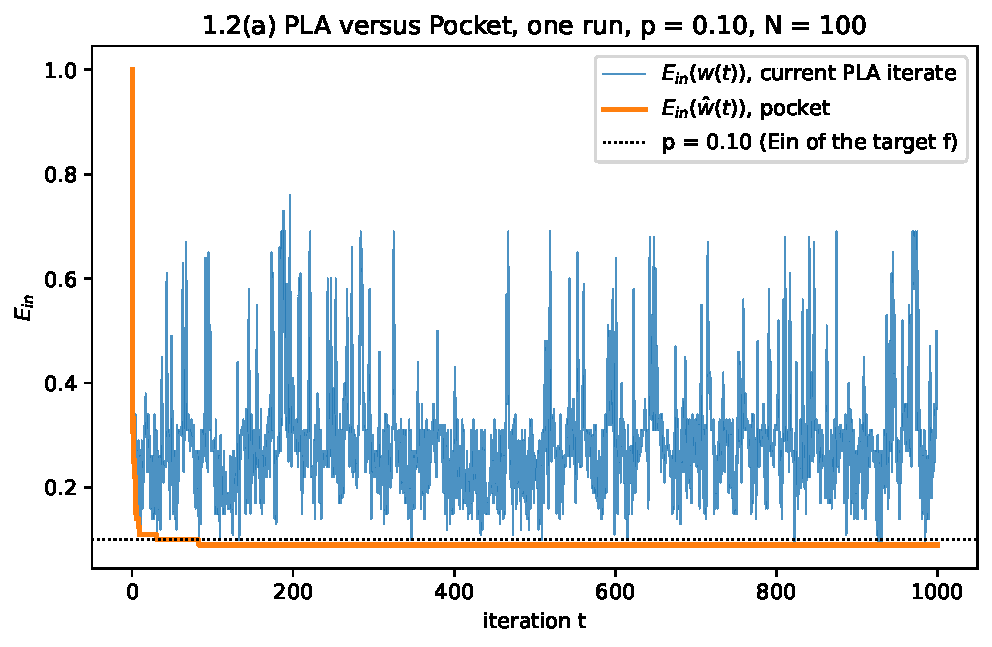
\includegraphics[width=0.255\textwidth]{fig_1_2a_ein_curves}\label{fig:p1a}}\hfil
\subfloat[]{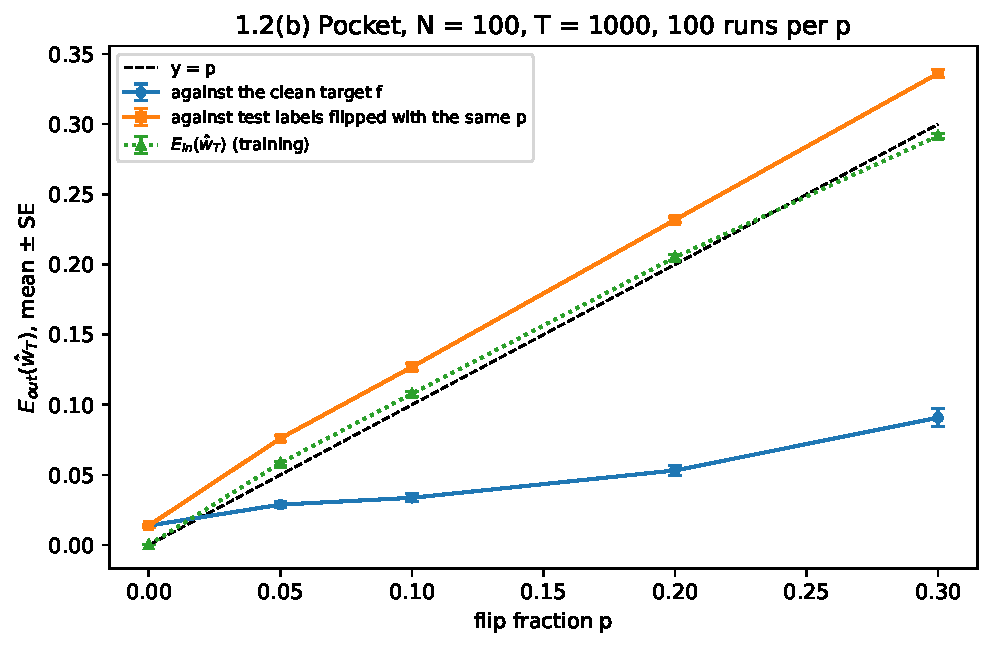
\includegraphics[width=0.255\textwidth]{fig_1_2b_eout_vs_p}\label{fig:p1b}}\hfil
\subfloat[]{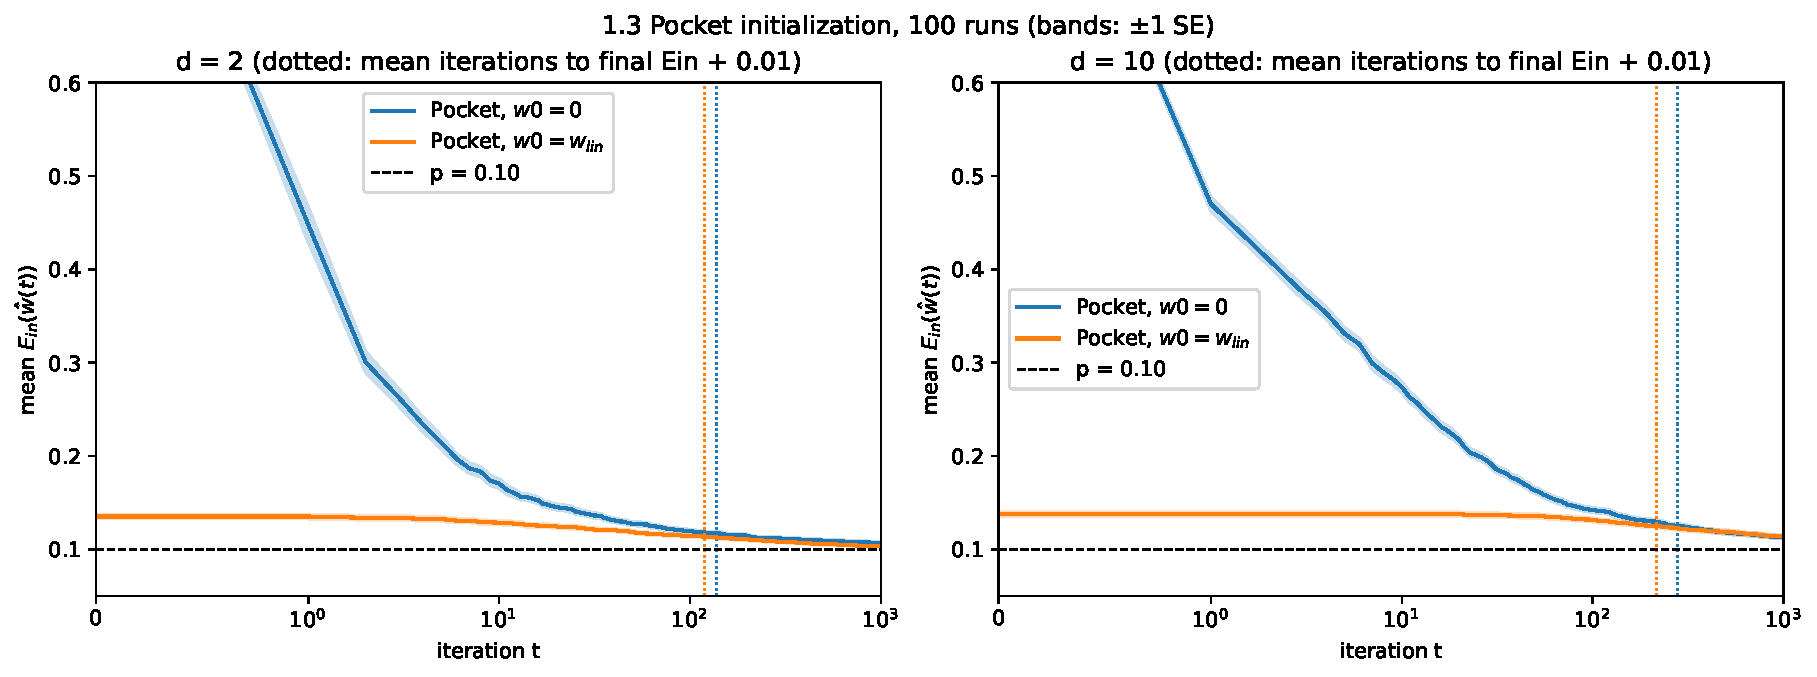
\includegraphics[width=0.47\textwidth]{fig_1_3_init}\label{fig:p1c}}
\caption{Part 1. (a) One run with $p=0.10$: the PLA iterate jumps, while Pocket's $\Ein(\hat\w(t))$ falls and ends below the target's own 0.10. (b) $\Eout(\hat\w_T)$ against the flip rate, measured against the clean $f$ and against flipped test labels, 100 runs per $p$. (c) Pocket started at $\w_0=0$ and at $\wlin$, $d=2$ and $d=10$, 100 runs (bands: $\pm1$ SE).}
\label{fig:p1}
\end{figure*}

\textbf{Simulated data (1.2).}
The first simulation, with \(10\%\) flipped labels, is shown in
Fig.~\ref{fig:p1}(a). The final error is \(\Ein=0.35\), so the PLA does not
converge. Pocket reduces the best error to \(0.09\), slightly below the
\(0.10\) obtained by \(f\).

Over 100 runs for each \(p\) (Fig.~\ref{fig:p1}(b)), the clean-label error is
\(0.034\pm0.003\) for \(p=0.10\) and \(0.091\pm0.007\) for \(p=0.30\).
Thus, the noise has little effect on the best line. When the test labels are
flipped using the same \(p\), the errors are \(0.127\pm0.002\) and
\(0.336\pm0.003\). They cannot be smaller than \(p\), because some labels are
intentionally incorrect. The expected error is

\[
\Eout^{\mathrm{flip}}
=
p+(1-2p)\Eout^{\mathrm{clean}}.
\]

\textbf{Convergence (1.2(c)).}
For separable data, PLA should reach \(\Ein=0\). With \(T=1000\) updates, it
failed in \(0.4\%\pm0.3\%\) of the 500 runs for \(N=100\), and in
\(21.4\%\pm1.8\%\) for \(N=1000\). The bound
\(R^2\lVert w^*\rVert^2/\rho^2\) increases from \(7.3\times10^4\) to
\(6.8\times10^6\), because more points are close to the decision boundary and
\(\rho\) becomes smaller. Although the bound is usually larger than \(T\),
the converged runs need only 58 and 421 updates. Therefore, it is a
worst-case estimate rather than the usual number of updates.

\textbf{Initialization (1.3).} Started at $\wlin$, Pocket begins at $\Ein\approx0.14$ instead of 1 (Fig.~\ref{fig:p1}(c)), so it needs fewer iterations to come within 0.01 of its final $\Ein$ (an absolute tolerance, since 1\% of 0.1 is below the $1/N$ resolution). It needs $119\pm18$ against $137\pm18$ for $d=2$, and $216\pm25$ against $278\pm23$ for $d=10$. The saving grows with $d$, from 18 to 62 iterations, because PLA builds its direction one point at a time while $\wlin$ costs one least-squares solve for any $d$. The final $\Ein$ is almost the same from both starts (0.1035 and 0.1072 for $d=2$), since the first PLA updates move away from $\wlin$ and only the stored pocket weights keep the advantage.

\begin{figure}[!t]
\centering
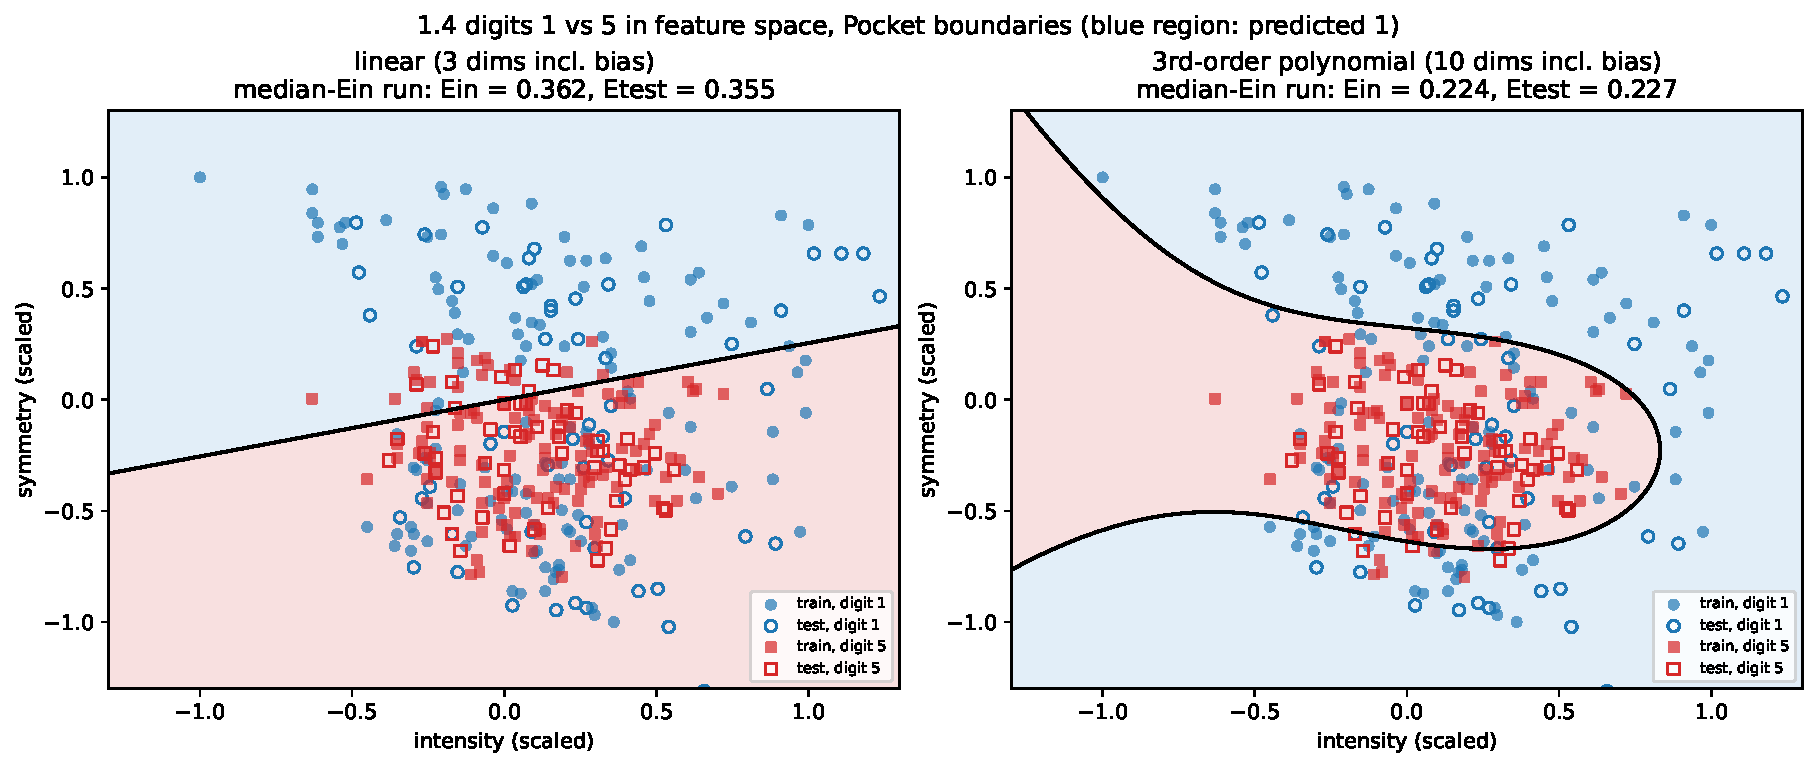
\includegraphics[width=\columnwidth]{fig_1_4_boundaries}
\caption{Digits 1 vs 5 (\texttt{load\_digits}) in the scaled intensity--symmetry plane, with the Pocket boundary of the median-$\Ein$ run for linear (left) and third-order polynomial (right) features.}
\label{fig:p1d}
\end{figure}

\textbf{Digits (1.4).}
The intensity and symmetry features are scaled to \([-1,1]\), using a
stratified \(70/30\) split of the \(8\times8\) \texttt{load\_digits} images.
The average intensities of digits 1 and 5 are \(0.302\) and \(0.300\).
Digit 5 forms a tight group, while digit 1 appears on both sides of it
(Fig.~\ref{fig:p1d}).

Over 100 Pocket runs, the linear model gives
\(\Ein=0.357\pm0.001\) and \(E_{\mathrm{test}}=0.352\pm0.002\). The cubic model with
10 weights gives \(\Ein=0.222\pm0.0004\) and
\(E_{\mathrm{test}}=0.2065\pm0.0011\), so it separates the digits better.

For 110 test points, the \(95\%\) Hoeffding margin is \(\epsilon=0.129\).
This gives \(\Eout\leq0.484\) for the linear model and
\(\Eout\leq0.357\) for the cubic model. For \(M=2\) models, the margin is
\(\epsilon=0.141\). The VC terms for \(d_{\mathrm{VC}}=3\) and \(10\) are
\(0.85\) and \(1.45\), so these bounds are not very useful.
We trust the cubic model more, because its test bound is lower and its \(E_{\mathrm{test}}\) shows no gap from \(\Ein\). Pocket itself only guarantees a low \(\Ein\), so any claim about \(\Eout\) has to come from a bound like this.

\subsection{Part 2: Linear regression}
\begin{figure*}[!t]
\centering
\subfloat[]{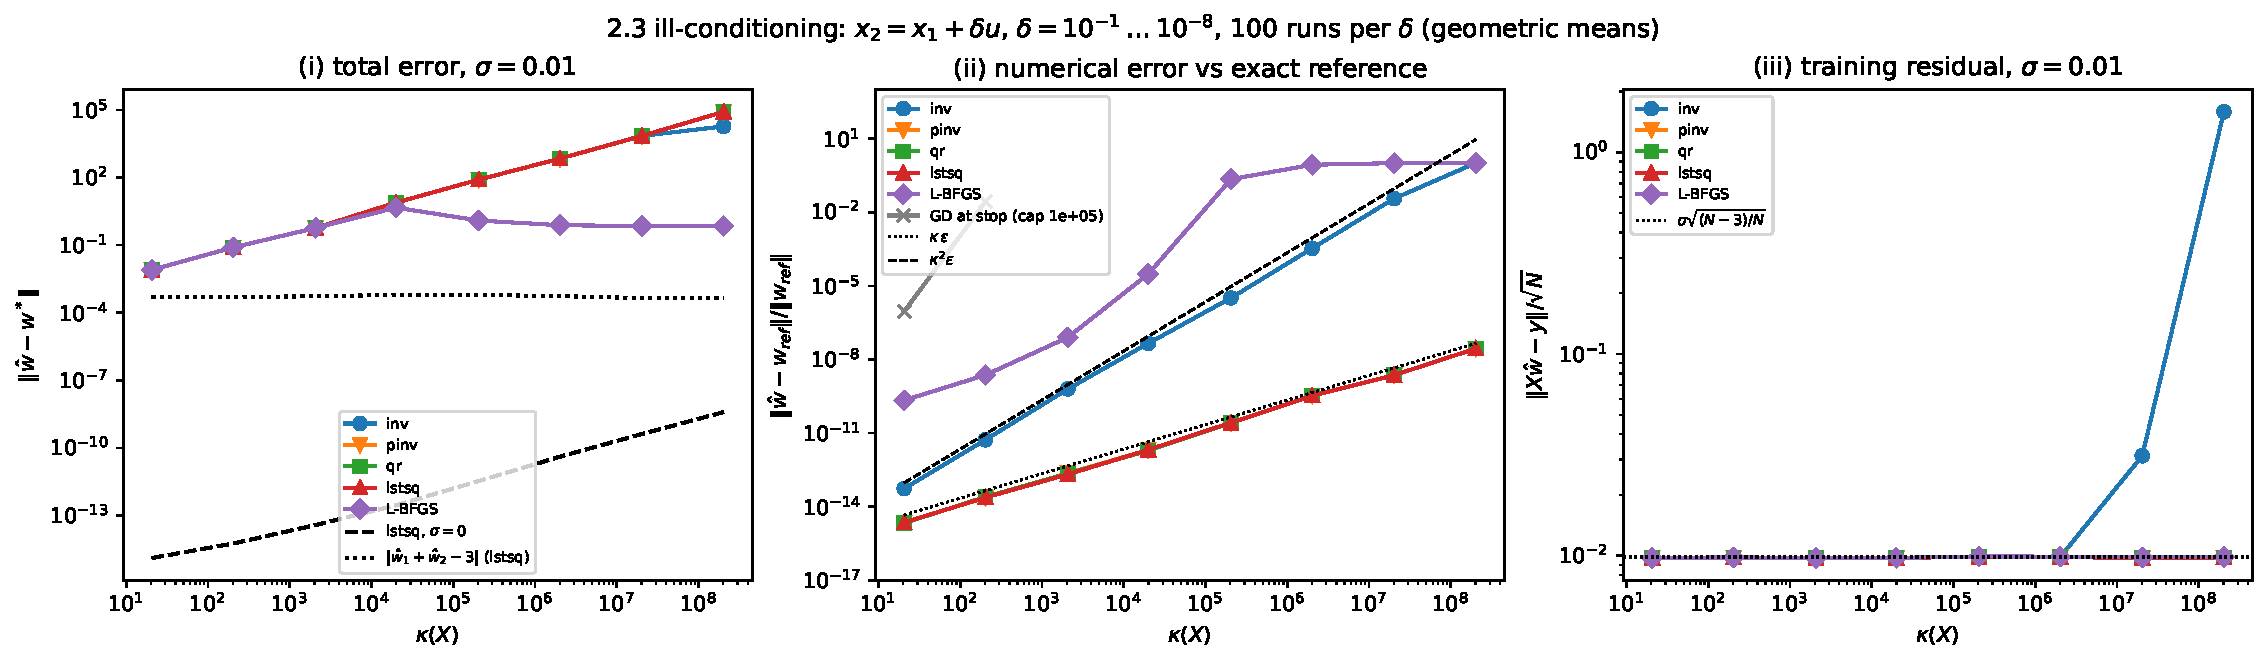
\includegraphics[width=0.655\textwidth]{fig_2_3_coef_error}\label{fig:p2a}}\hfil
\subfloat[]{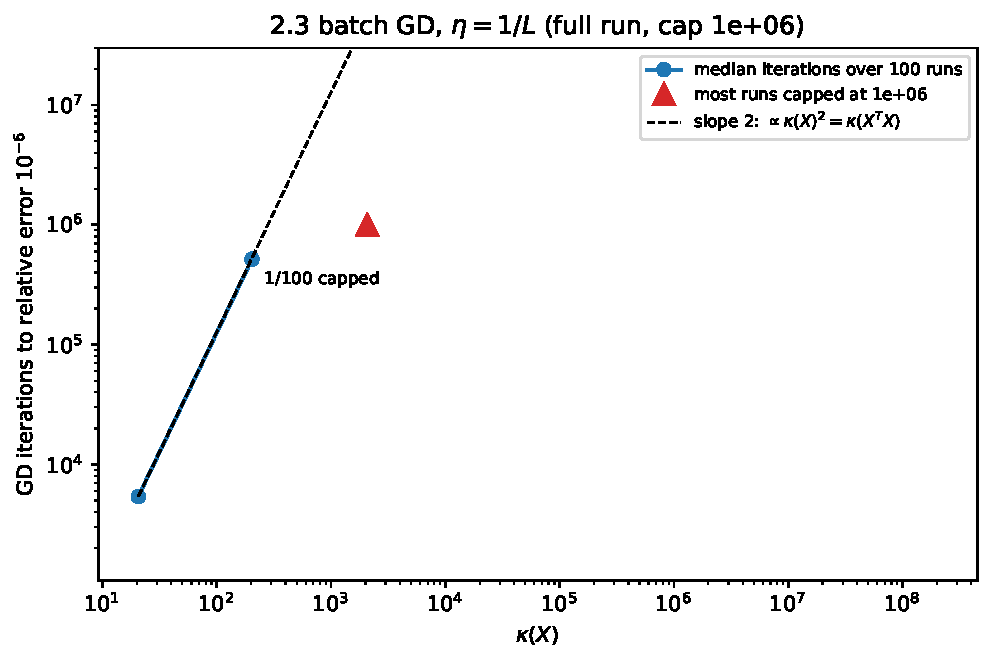
\includegraphics[width=0.315\textwidth]{fig_2_3_gd_iterations}\label{fig:p2b}}\\
\subfloat[]{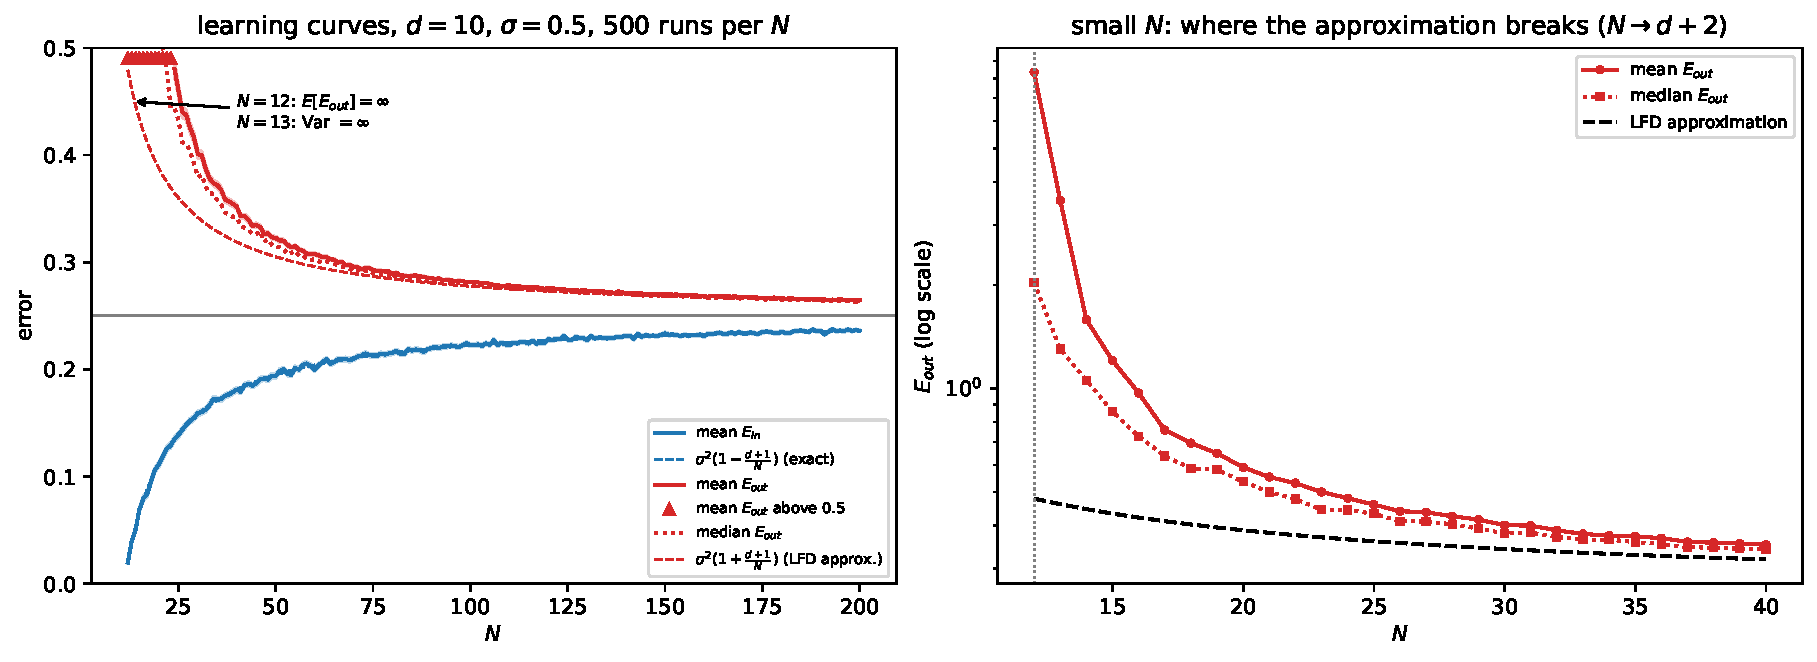
\includegraphics[width=0.49\textwidth]{fig_2_4_learning_curves}\label{fig:p2c}}\hfil
\subfloat[]{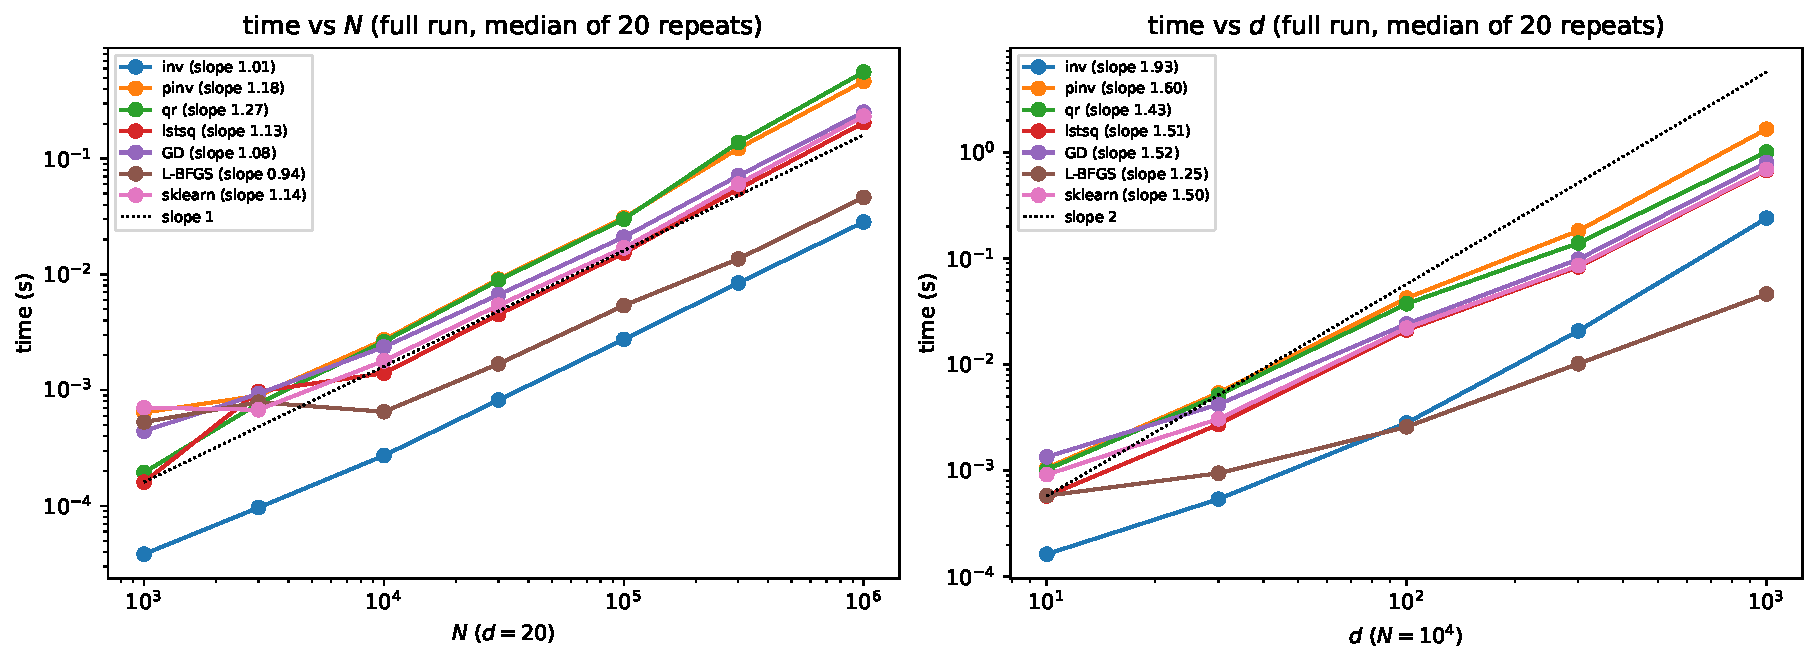
\includegraphics[width=0.49\textwidth]{fig_2_6_timing}\label{fig:p2d}}
\caption{Part 2. (a) Coefficient error and residual of the five solvers against $\kappa(\X)$ (100 runs per $\delta$). (b) Gradient-descent iterations to a relative error of $10^{-6}$ against $\kappa(\X)$. (c) Learning curves, $d=10$, 500 runs per $N$, with LFD's formulas. (d) Solver timing against $N$ ($d=20$) and $d$ ($N=10^4$), single BLAS thread, median of 20 repeats.}
\label{fig:p2}
\end{figure*}

\textbf{Solvers and conditioning (2.2, 2.3).} The gradient check passes ($3.4\times10^{-10}$), and all five solvers agree with \texttt{lstsq} to $\le1.4\times10^{-9}$ on a well-conditioned problem. With $x_2=x_1+\delta u$, the condition number grows from 21 to $2\times10^8$ as $\delta$ goes from $10^{-1}$ to $10^{-8}$. We measure each solver's numerical error against an exact reference computed in the well-conditioned basis $[1,x_1,u]$ (Fig.~\ref{fig:p2}(a)). QR, SVD and \texttt{lstsq} track $\kappa\epsilon_{\mathrm{mach}}$, reaching $2.8\times10^{-8}$ at the largest $\kappa$. \texttt{inv} tracks $\kappa^2\epsilon_{\mathrm{mach}}$ and reaches 100\% relative error at $\kappa=2\times10^8$. L-BFGS stalls from $\kappa\approx2\times10^5$. The statistical error $\lVert\hat\w-\w^*\rVert$ also grows by orders of magnitude with $\kappa$, even for exact solvers, but $w_1+w_2$ stays determined to about $5\times10^{-4}$ at every $\delta$. Only the direction along $x_1-x_2$ is lost. Gradient descent needs 5\,400 iterations at $\kappa=20.6$ and 516\,600 at $\kappa=203$, a ratio of 95.7 against the predicted $\kappa^2$ ratio of 97.7 (Fig.~\ref{fig:p2}(b)). We would ship QR or \texttt{lstsq}. The lecture formula with \texttt{inv} squares $\kappa$ before solving, which is why its error reached 100\% at $\kappa=2\times10^8$.

\textbf{Learning curves (2.4).} The $\Ein$ formula is exact. Over 189 values of $N$ the largest deviation is 2.7 SE (median 0.5). The $\Eout$ approximation is not. It underestimates by 18 SE at $N=20$ and still by 3.6 SE at $N=200$ (Fig.~\ref{fig:p2}(c)). Near $N=d+1$, rare and nearly singular designs dominate the mean. At $N=12$ the mean $\Eout$ is $8.3\pm2.1$ while the median is 2.0. The approximation fails there because $E[(\X\T\X)^{-1}]$ grows like $1/(N-d-2)$ rather than $1/N$.

\textbf{California housing (2.5).}
The test MSE is \(0.515\pm0.018\), the training MSE is \(0.527\), and the test
\(R^2\) is \(0.605\). Since the training and test errors are close, there is
no obvious overfitting. The model uses 9 weights and 16,512 data points.

The target is limited to \(\$500{,}000\) for \(5\%\) of the districts, which
are underestimated by \(1.08\) on average. The standardized coefficients are
\(-0.91\) for latitude, \(-0.88\) for longitude, and \(+0.83\) for income.
Latitude and longitude have correlation \(-0.93\), so they mainly describe
location relative to the coast. \texttt{AveRooms} and \texttt{AveBedrms}
have correlation \(+0.86\), but their coefficients have opposite signs.
Therefore, coefficients of correlated features are conditional effects and
should not be treated as direct causal effects.

\textbf{Timing (2.6).} In $N$ every solver scales with slope 0.94--1.27, consistent with $O(Nd^2)$ for the direct methods (Fig.~\ref{fig:p2}(d)). In $d$ only \texttt{inv} reaches the predicted slope 2 (1.93); the others reach 1.25--1.60, because BLAS-3 kernels become more efficient as matrices grow. \texttt{inv} is also the fastest at $N=10^6$ (0.028\,s, against 0.20\,s for \texttt{lstsq}), but 2.3 shows that it is the least accurate.

\textbf{Linear regression for classification (2.7).} On the 1.4 digits, $\mathrm{sign}(\wlin\T\x)$ has $\Ein=0.421$ against Pocket's $0.355$. Squared loss also penalizes correct points far from the boundary, so the fitted line sits between the two groups of 1s. It is still a useful starting point, and Pocket from $\wlin$ ends at $\Ein=0.349$ and $E_{\mathrm{test}}=0.340$.

\subsection{Part 3: Logistic regression}
\begin{figure*}[!t]
\centering
\subfloat[]{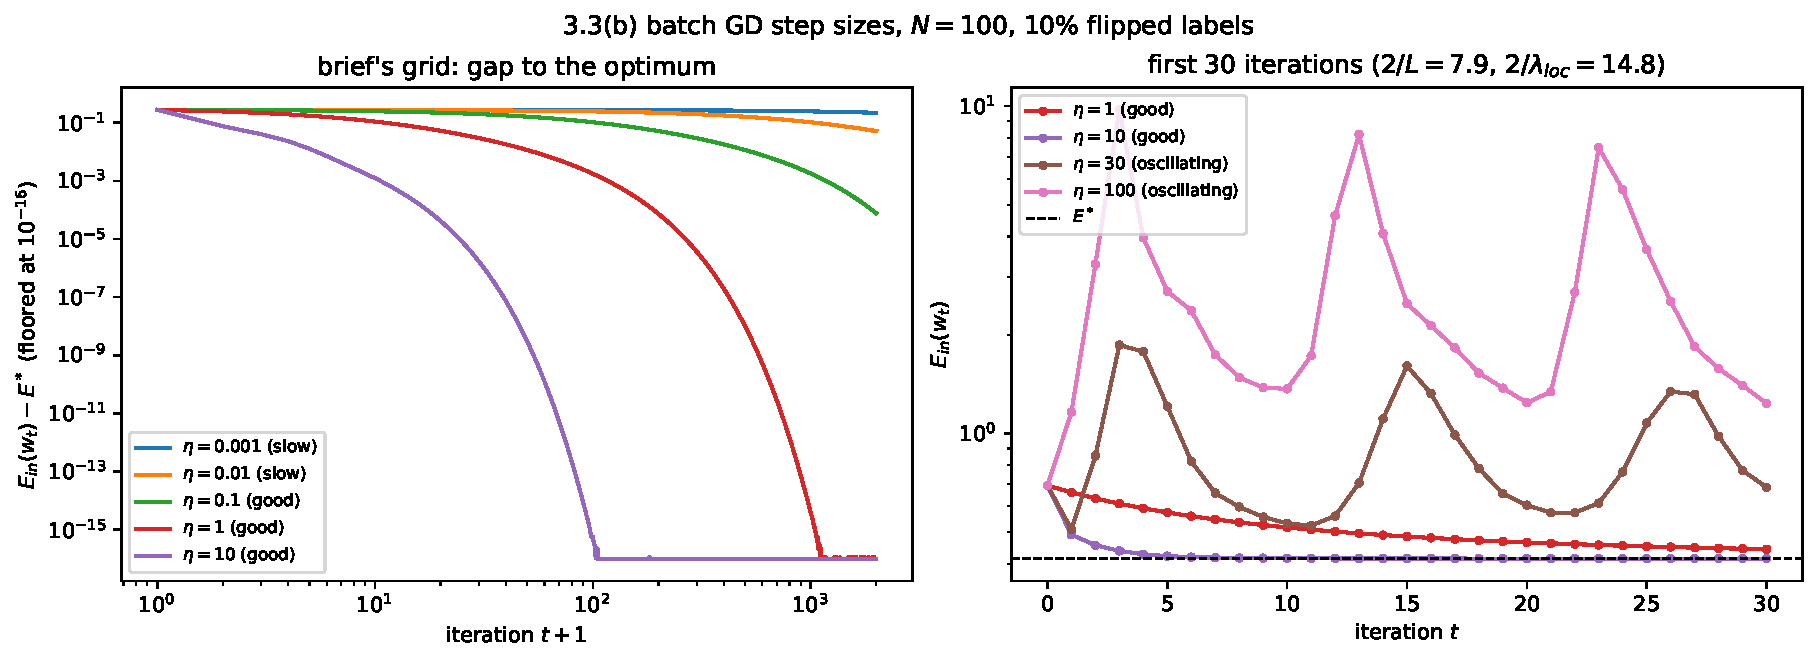
\includegraphics[width=0.49\textwidth]{fig_3_3b_step_sizes}\label{fig:p3a}}\hfil
\subfloat[]{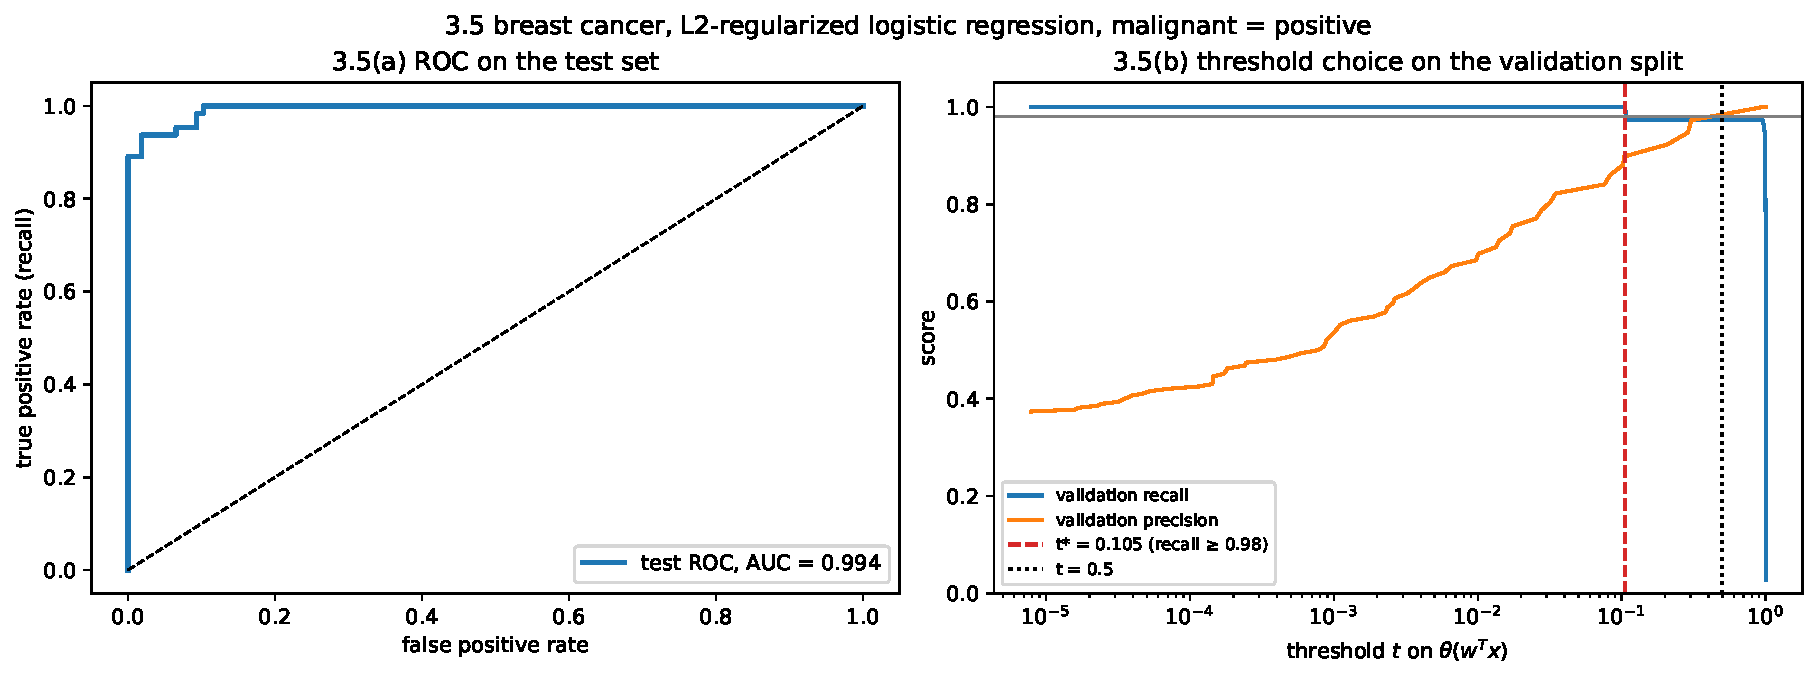
\includegraphics[width=0.49\textwidth]{fig_3_5_roc_threshold}\label{fig:p3b}}\\
\subfloat[]{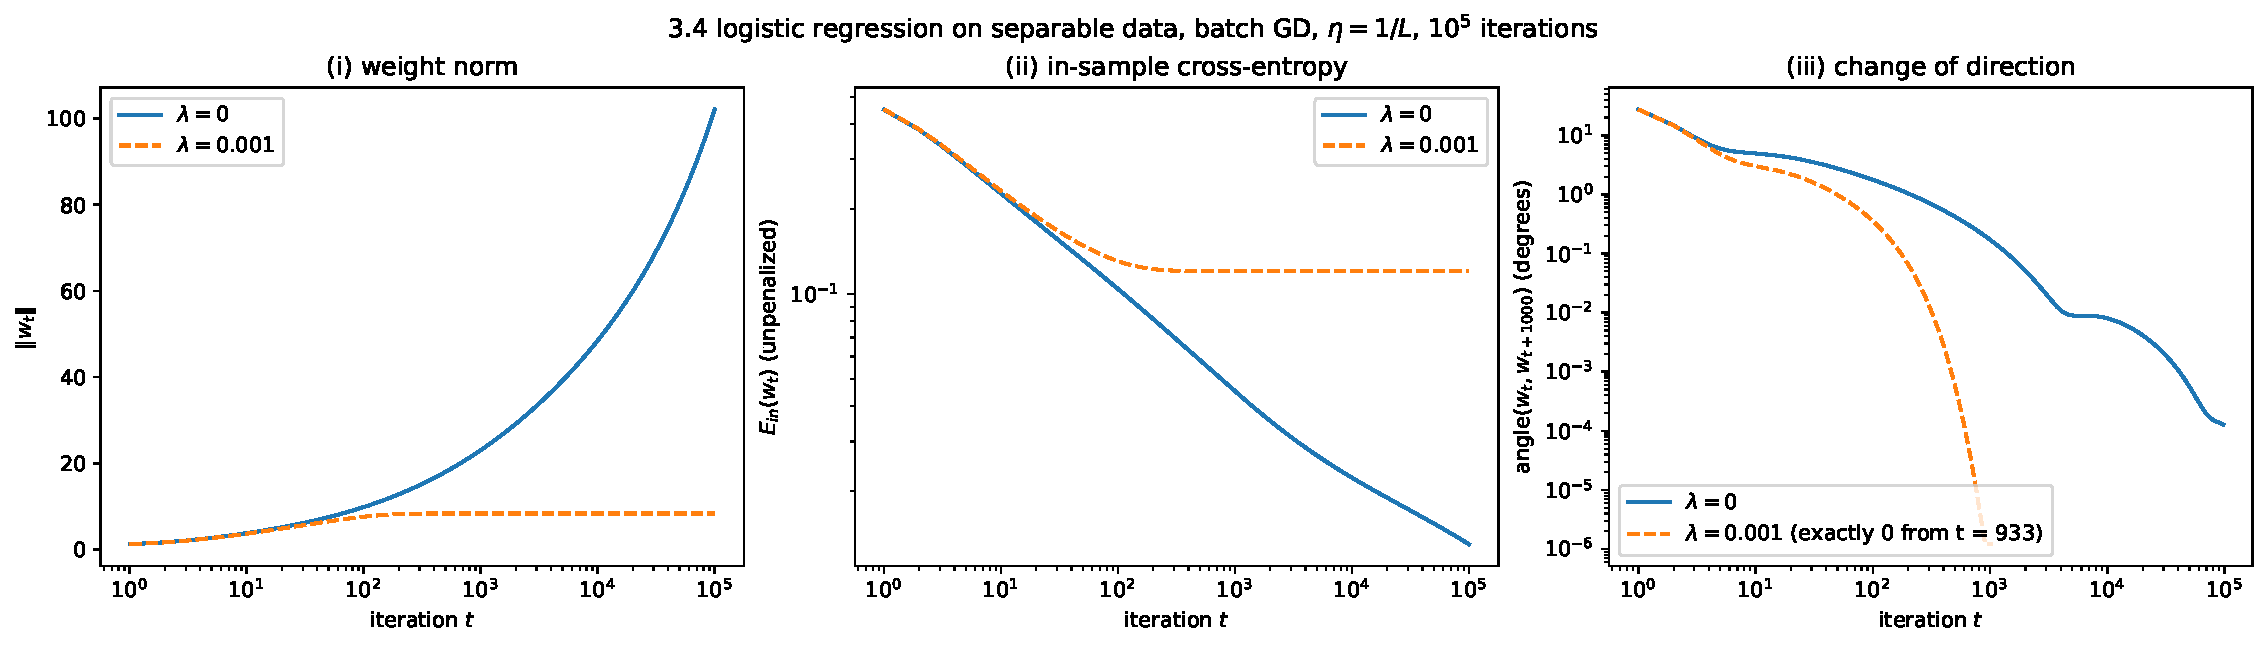
\includegraphics[width=0.6\textwidth]{fig_3_4_separable}\label{fig:p3c}}
\caption{Part 3. (a) Batch GD on noisy data for $\eta$ from $10^{-3}$ to 100. (b) Breast cancer: test ROC and the choice of a recall-$\ge0.98$ threshold on a validation split. (c) Separable data: $\lVert\w_t\rVert$, $\Ein(\w_t)$ and the angle between $\w_t$ and $\w_{t+1000}$, without and with L2 ($\lambda=10^{-3}$).}
\label{fig:p3}
\end{figure*}

\textbf{Stability and optimizers (3.2, 3.3).} At $s=\pm1000$ the stable $\Ein$ returns exactly 500 with no warnings, where the naive formula overflows to \texttt{inf}. With $\eta=0.01$ and the brief's stopping rule, SGD needs $333\pm5$ epochs and reaches a cross-entropy $\Eout$ of $0.102\pm0.001$ (100 runs). To give the optimum a finite value, we flip 10\% of the labels for the step-size sweep (Fig.~\ref{fig:p3}(a)). After 2\,000 iterations, $\eta\le10^{-2}$ is still 0.05--0.22 above $E^*$ (slow), $\eta=1$ and $10$ have converged (good), and $\eta=30$ and $100$ oscillate, with 992 and 597 increases of $\Ein$. $\eta=10$ exceeds the global bound $2/L=7.9$ but not the local one at the optimum, $2/\lambda_{\max}(\nabla^2\Ein(\w^*))=14.8$. To reach $E^*+10^{-6}$, L-BFGS needs 11 iterations (about 0.3\,ms) and gradient descent 31 at $\eta=10$ (about 0.3\,ms). SGD needs 344 epochs at $\eta=0.01$ (about 0.1\,s) and 1\,494 at $\eta=0.1$ (about 0.45\,s). With a constant step, SGD's gradient noise sets a floor that grows with $\eta$, so the larger step is slower.

\textbf{Separable data (3.4).} Without a penalty, $\lVert\w_t\rVert$ grows from 23 to 102 over $10^5$ iterations, $\Ein$ keeps falling from 0.045 to 0.013, and every predicted probability moves towards 0 or 1 (Fig.~\ref{fig:p3}(c)). No finite minimizer exists, yet the angle between $\w_t$ and $\w_{t+1000}$ shrinks from $0.17^\circ$ to $1.3\times10^{-4\,\circ}$, so the direction converges. Gradient descent on separable data converges in direction to the max-margin separator~\cite{soudry2018}, the SVM solution. With $\lambda=10^{-3}$ the norm stops at $8.37$, $\Ein$ plateaus at $0.120$, and all three curves become flat.

\textbf{Breast cancer (3.5).}
The malignant class is target 0, with a stratified \(70/30\) split. The
training data are linearly separable, so logistic regression has no finite
optimum without regularization. Using 10-fold cross-validation, the L2
regularization value was selected as
\(\lambda^*=1.8\times10^{-3}\).

At threshold \(0.5\), the test results are
\(\mathrm{accuracy}=0.953\), \(\mathrm{precision}=0.967\),
\(\mathrm{recall}=0.906\), \(F1=0.936\), and \(\mathrm{AUC}=0.994\).
The model misses 6 of 64 malignant tumors and gives 2 false alarms.

The largest validation threshold satisfying
\(\mathrm{recall}\geq0.98\) is \(t^*=0.105\). With 37 malignant validation
cases, one missed case changes the recall by \(1/37=0.027\). On the test set,
this threshold gives recall \(0.953\) and precision \(0.859\), compared with
\(0.922\) and \(0.983\) at threshold \(0.5\). It misses two fewer cancers but
produces nine additional false alarms (Fig.~\ref{fig:p3}(b)). Therefore,
threshold \(0.5\) is not optimal when missing a cancer is much more serious
than requiring an additional examination.

\subsection{Part 4: Overfitting and regularization}
\begin{figure*}[!t]
\centering
\subfloat[]{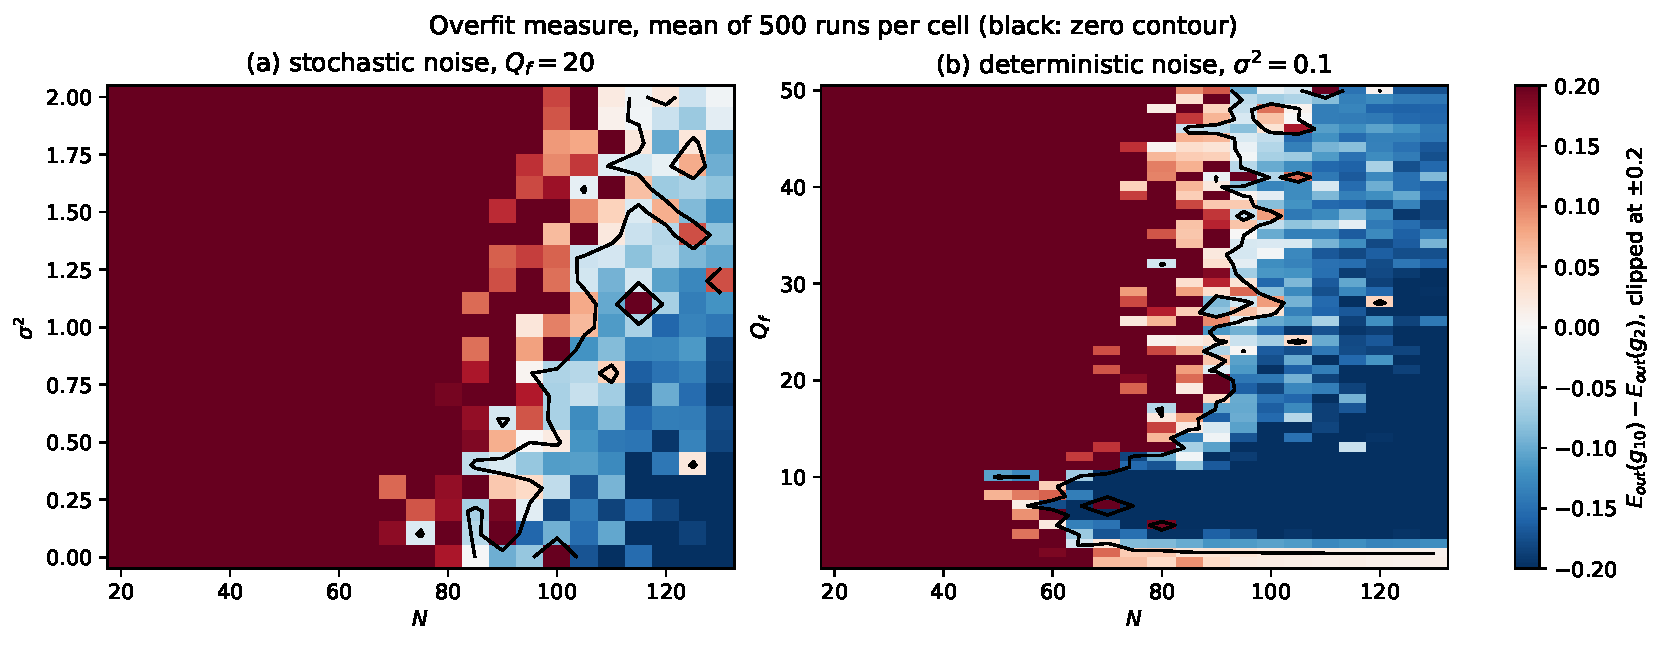
\includegraphics[width=0.66\textwidth]{fig_4_1c_heatmaps}\label{fig:p4a}}\\
\subfloat[]{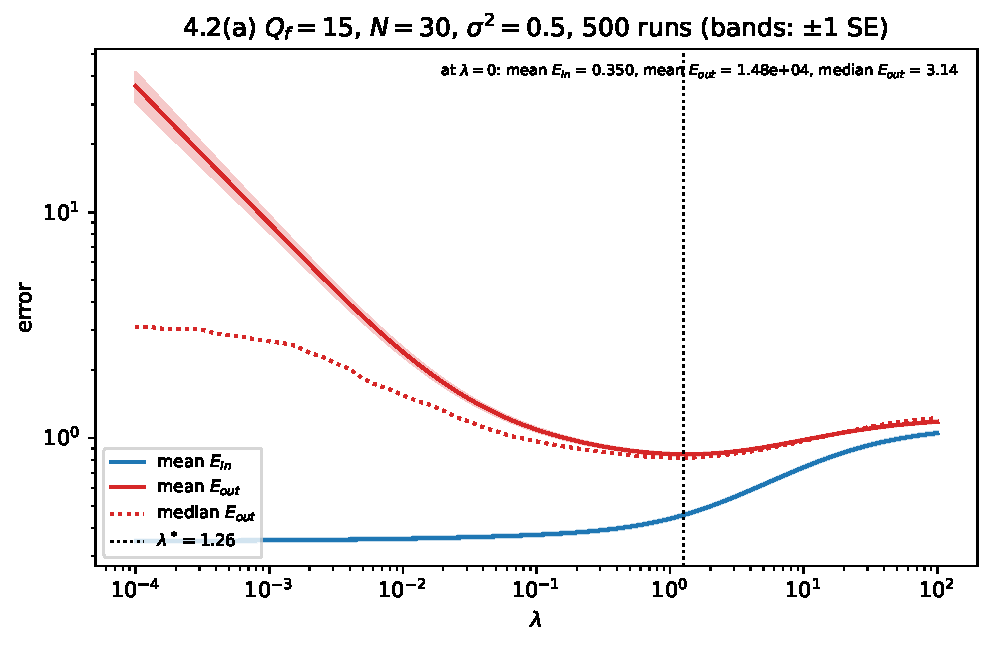
\includegraphics[width=0.325\textwidth]{fig_4_2a_lambda_sweep}\label{fig:p4c}}\hfil
\subfloat[]{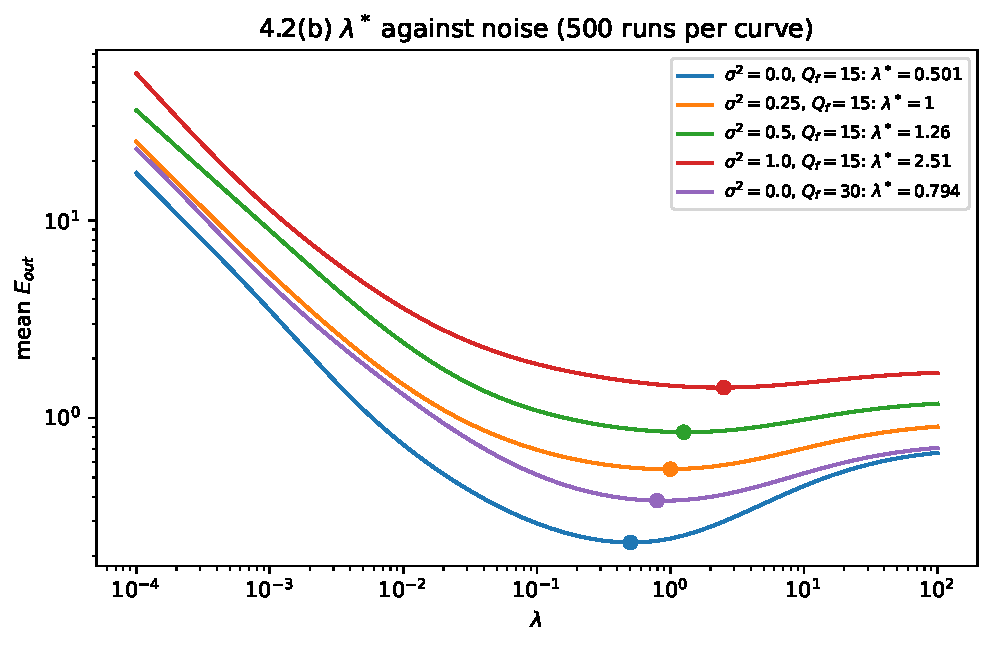
\includegraphics[width=0.325\textwidth]{fig_4_2b_noise_lambda_star}\label{fig:p4d}}\hfil
\subfloat[]{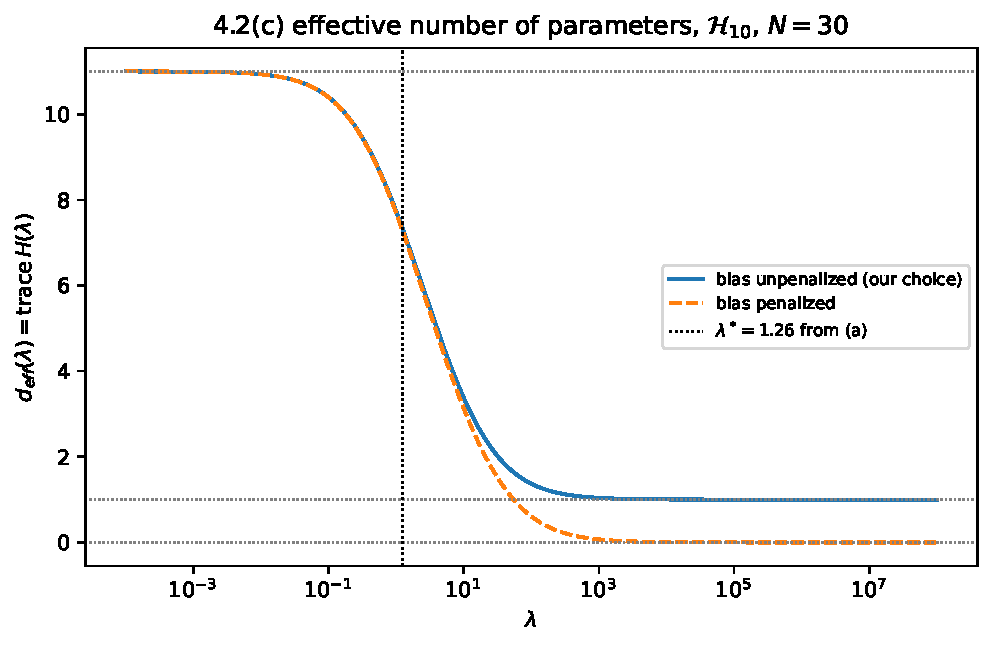
\includegraphics[width=0.325\textwidth]{fig_4_2c_deff}\label{fig:p4e}}
\caption{Part 4. (a) Overfit measure $\Eout(g_{10})-\Eout(g_2)$ against $N$ and $\sigma^2$ ($Q_f=20$), and against $N$ and $Q_f$ ($\sigma^2=0.1$), with 500 runs per cell and analytic $\Eout$. (b) Weight decay, $Q_f=15$, $N=30$, $\sigma^2=0.5$, 500 runs. (c) $\Eout(\lambda)$ for four noise levels and the deterministic case. (d) $d_{\mathrm{eff}}(\lambda)$.}
\label{fig:p4}
\end{figure*}

\textbf{Overfitting (4.1).} With the analytic $\Eout$ \eqref{eq:eout} and fits batched over runs, both heatmaps (Fig.~\ref{fig:p4}(a)) show overfitting at small $N$, and its boundary moves to larger $N$ as either kind of noise grows. With stochastic noise, the first $N$ at which the median overfit measure turns negative moves from 40 ($\sigma^2=0$) to 95 ($\sigma^2=2$). With deterministic noise it moves from 30 ($Q_f=10$) to 40 ($Q_f=20$) and 55 ($Q_f=50$).
When $\sigma^2$ is small, $\mathcal H_{10}$ fits the part of $f$ it cannot represent. On 20--50 random points, $L_{11},\dots,L_{Q_f}$ are not orthogonal to the low orders, so least squares aliases them into wrong low-order coefficients. For $Q_f\le2$ the target lies inside $\mathcal H_2$, and $\mathcal H_{10}$ overfits at every $N$. Rare runs that swing far from $f$ near $x=\pm1$ dominate the mean. At $N=20$ the mean overfit measures reach $10^4$--$10^8$ while the medians are 4--70.

\textbf{Weight decay (4.2).} $\Ein$ rises with $\lambda$ while $\Eout$ is U-shaped, with its minimum $0.848\pm0.008$ at $\lambda^*=1.26$ (Fig.~\ref{fig:p4}(b)). At $\lambda=0$ the mean $\Eout$ is $1.5\times10^4$ (median 3.1); even a small $\lambda$ removes that tail, because \eqref{eq:ridge} replaces $1/s_i$ by $s_i/(s_i^2+\lambda)$ on the near-singular directions. Noise of either kind moves $\lambda^*$ up (Fig.~\ref{fig:p4}(c)). It grows from $0.50$ to $1.0$, $1.26$ and $2.51$ as $\sigma^2$ goes from 0 to 1. With no stochastic noise it is still positive, $0.50$ for $Q_f=15$ and $0.79$ for $Q_f=30$, because of the deterministic noise. $d_{\mathrm{eff}}$ falls from exactly 11 to its limit of 1 with an unpenalized bias, or 0 with a penalized one (Fig.~\ref{fig:p4}(d)); at $\lambda^*$ it is 7.30. On a single dataset, the under-, well- and over-regularized fits at $\lambda=0$, $1.26$ and $100$ give $\Eout=8710$, $0.771$ and $1.063$. We leave the bias unpenalized. Shifting $y$ by 3 leaves that model unchanged ($0.848$), while the penalized model worsens to $6.66$ at $\lambda=100$, and a learning method should not depend on the origin of $y$.

\begin{figure*}[!t]
\centering
\subfloat[]{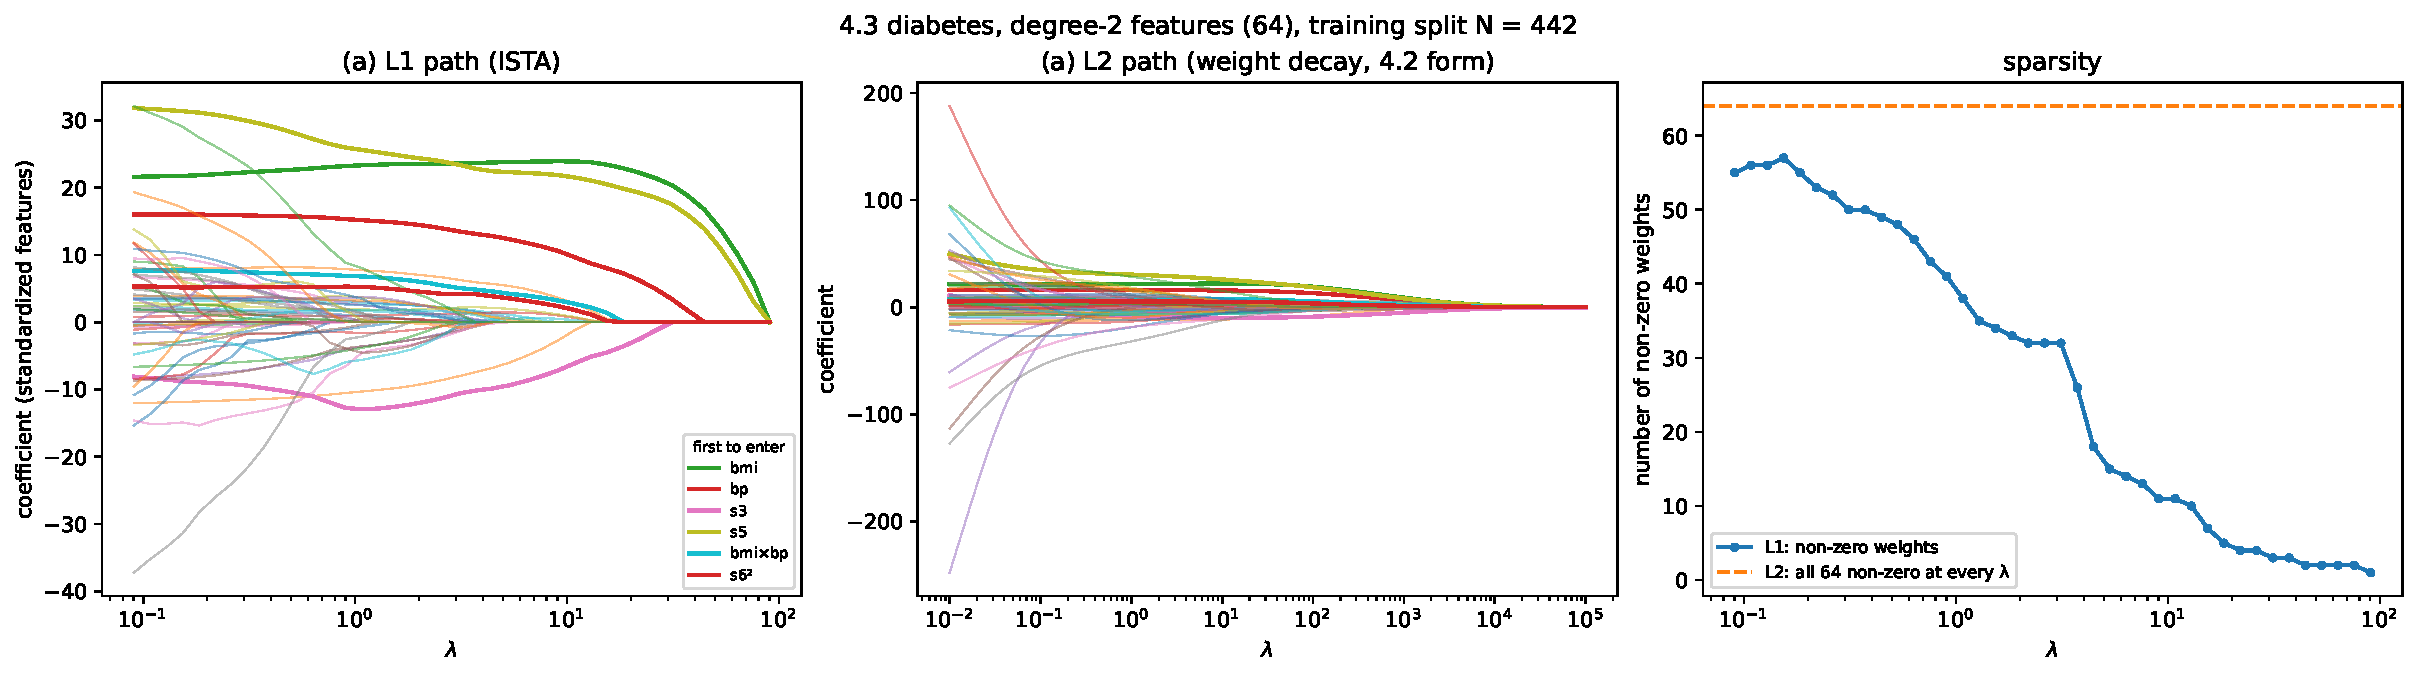
\includegraphics[width=0.76\textwidth]{fig_4_3a_paths}\label{fig:p4f}}\\
\subfloat[]{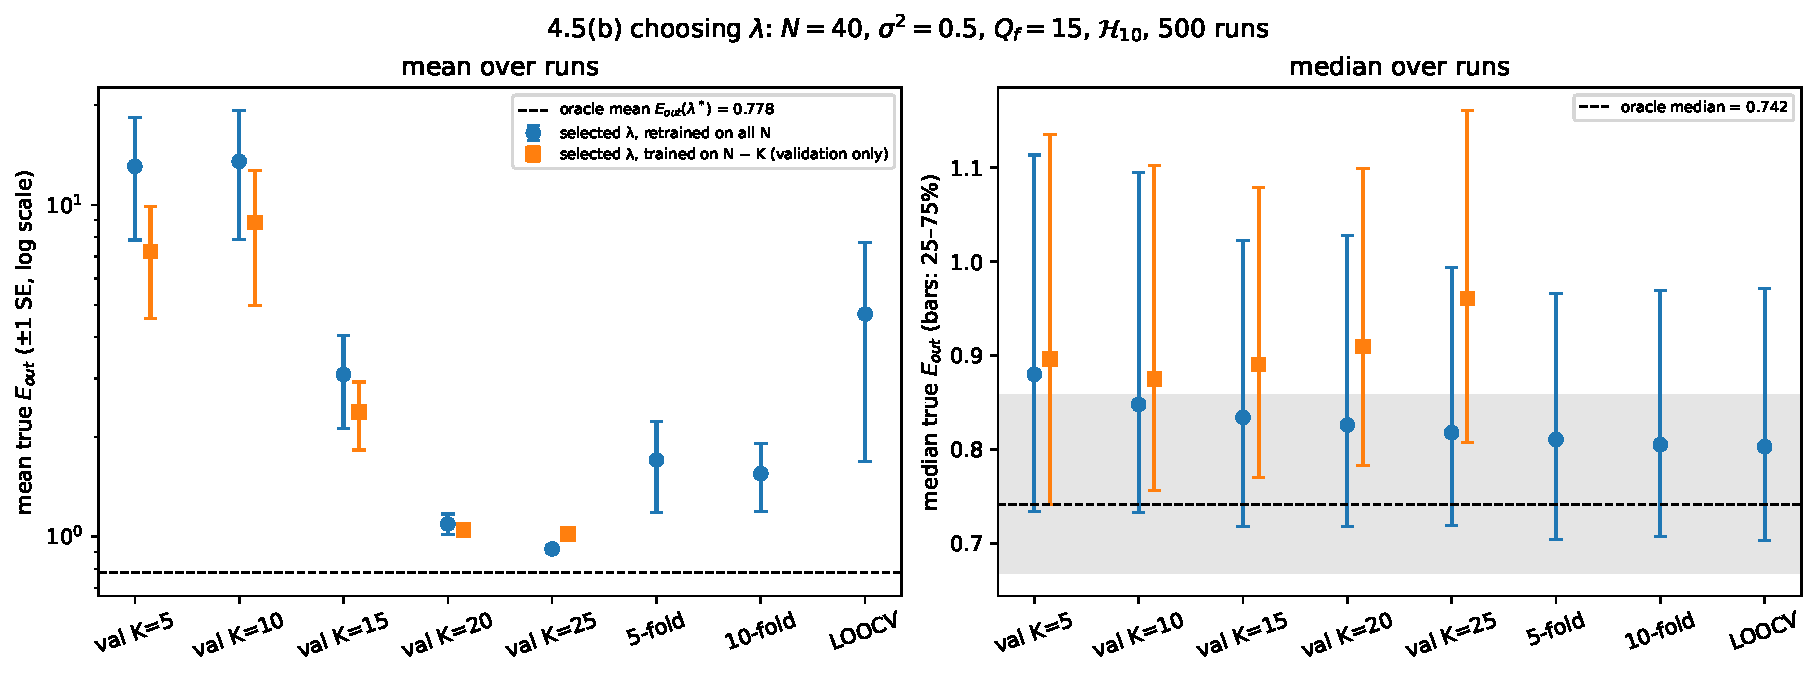
\includegraphics[width=0.56\textwidth]{fig_4_5b_selection}\label{fig:p4g}}\hfil
\subfloat[]{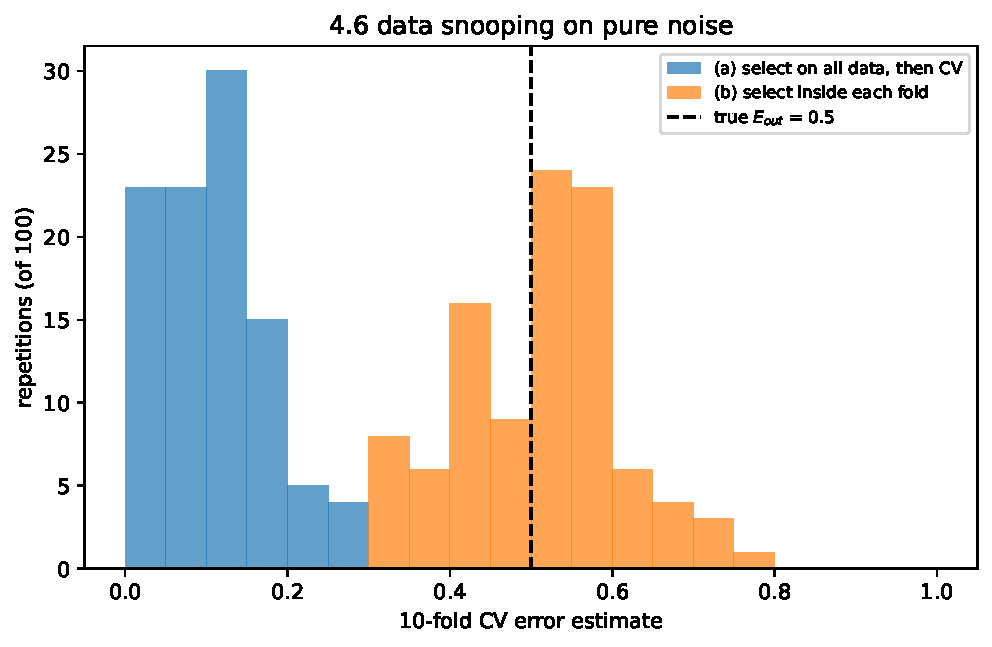
\includegraphics[width=0.35\textwidth]{fig_4_6_snooping}\label{fig:p4h}}
\caption{Part 4, continued. (a) Diabetes, degree-2 features: L1 and L2 paths and the number of non-zero weights. (b) Selecting $\lambda$ for weight decay ($N=40$, 500 runs): $\Eout$ of the selected model for each method against the oracle. (c) Data snooping on pure noise, 100 repetitions: 10-fold CV error with feature selection on all data and inside each fold.}
\label{fig:p4b2}
\end{figure*}

\textbf{Sparsity (4.3).} We use all 442 diabetes patients with degree-2 features. Since sex is binary, $\mathrm{sex}^2$ is affine in sex and is dropped, leaving 64 standardized features. L1 weights enter one at a time (Fig.~\ref{fig:p4b2}(a)), first body-mass index, serum triglycerides (s5) and blood pressure, while L2 keeps all 64 non-zero at every $\lambda$. Geometrically, the L1 ball has corners on the axes where a contour of $\Ein$ first touches it. Algebraically, $S_{\eta\lambda}$ in \eqref{eq:ista} maps every $|v_j|\le\eta\lambda$ to exactly zero, whereas weight decay only scales each direction by $s_i^2/(s_i^2+\lambda)>0$. ISTA needs a median of 1726 iterations per $\lambda$, because its step is set by the largest curvature of a matrix with $\kappa=5470$.

\textbf{Regularized logistic regression (4.4).} Breast cancer with degree-2 features (495) and $N_{\mathrm{train}}=100$ is separable, so at $\lambda=0$ L-BFGS stops at an arbitrary point when its tolerance test passes (test error 0.062). With 5-fold CV on the training points, L2 selects $\lambda^*=0.631$ (test error 0.049) and L1 selects $\lambda^*=0.018$ (test error 0.041) with 18 of 495 features. The survivors are products of tumour size, texture, smoothness and concave points, the features clinicians associate with irregular, enlarged nuclei~\cite{street1993}.

\textbf{Validation (4.5).} The closed form \eqref{eq:loocv} matches brute-force LOO refits to $6\times10^{-13}$ (unpenalized bias) and $1.3\times10^{-12}$ (penalized) over 62 values of $\lambda$. It costs one SVD instead of $N$ fits, and at $N=1600$ it is about three orders of magnitude faster. Table~\ref{tab:cv} compares the selection methods.
\begin{itemize}
\item In the typical run, $K$-fold and LOO do best, with medians of 0.80--0.81 against the oracle's 0.74.
\item The means are dominated by rare catastrophic choices of a tiny $\lambda$, which hit small validation sets most often.
\item The validation error of the selected model is optimistic in 65--81\% of runs. We report the minimum of 62 noisy estimates, and $E[\min_\lambda E_{\mathrm{val}}]\le\min_\lambda E[E_{\mathrm{val}}]$.
\end{itemize}

\begin{table}[!t]
\caption{Selecting $\lambda$ for weight decay, $N=40$, 500 runs (oracle: mean $0.778\pm0.007$, median $0.742$). Last column: share of runs with $\Eout$ above twice the oracle's.}
\label{tab:cv}
\centering\footnotesize
\begin{tabular}{lccc}
\toprule
Method & mean $\Eout$ & median & $>2\times$ oracle\\
\midrule
validation, $K=5$ & $13.1\pm5.2$ & 0.880 & 10.8\%\\
validation, $K=25$ & $0.918\pm0.024$ & 0.818 & 2.4\%\\
5-fold CV & $1.70\pm0.52$ & 0.811 & 4.6\%\\
10-fold CV & $1.55\pm0.36$ & 0.805 & 5.0\%\\
LOOCV & $4.69\pm3.00$ & 0.803 & 5.8\%\\
\bottomrule
\end{tabular}
\end{table}

\textbf{Data snooping (4.6).} The data are pure noise: 50 points, 1000 Gaussian features and coin-flip labels, so every classifier has $\Eout=0.5$. Choosing the 20 features most correlated with the labels on all the data, and then cross-validating, reports an error of $0.103\pm0.006$; it is below 0.3 in all 100 repetitions (Fig.~\ref{fig:p4b2}(c)). Choosing inside each fold reports $0.508\pm0.010$. The selected features have $|{\rm corr}|=0.37$ against a typical $1/\sqrt N=0.14$, because the selection step saw the validation points. The same leak could have entered our 3.5, 4.3 and 4.4 had the standardization been fitted before splitting into folds, so every fold refits its own.

\subsection{Part 5: The digits challenge}
\begin{figure*}[!t]
\centering
\subfloat[]{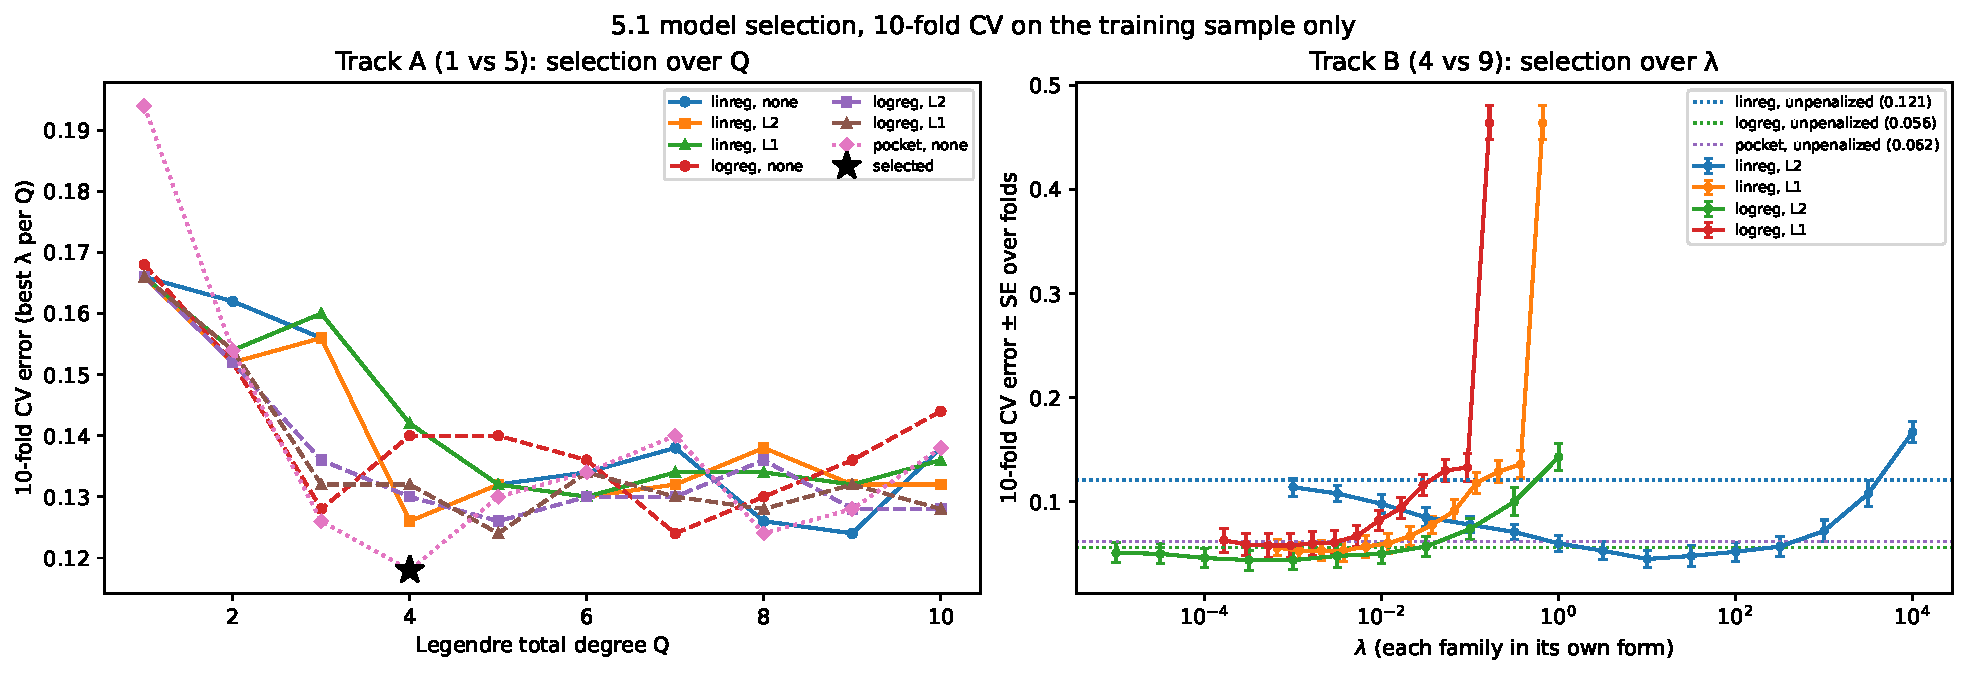
\includegraphics[width=0.64\textwidth]{fig_5_1_selection}\label{fig:p5a}}\hfil
\subfloat[]{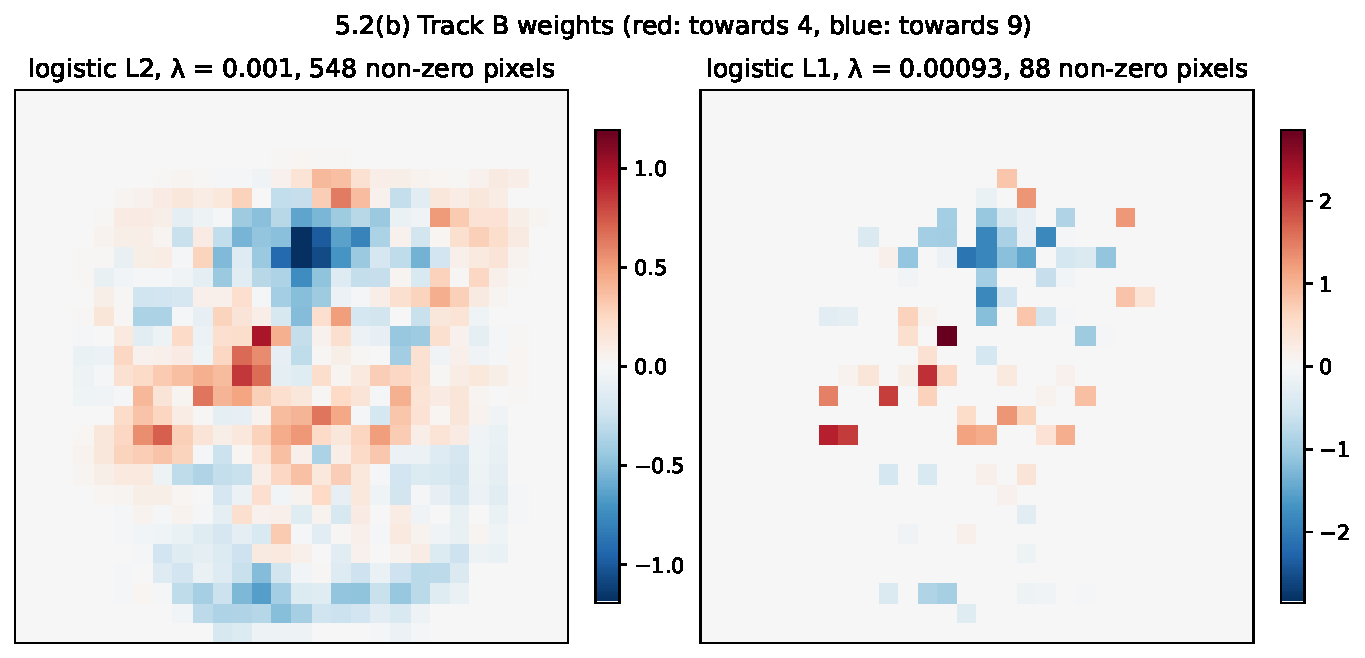
\includegraphics[width=0.31\textwidth]{fig_5_2b_track_b_weights}\label{fig:p5b}}
\caption{Part 5. (a) 10-fold CV error of every candidate: Track A against the Legendre degree $Q$, Track B against $\lambda$. (b) Track B weights as $28\times28$ images (red: towards 4, blue: towards 9), each at its own CV-selected $\lambda$.}
\label{fig:p5}
\end{figure*}

MNIST is split into the first 60\,000 images as the training pool and the last 10\,000 as the test set.
\begin{itemize}
\item \textbf{Track A} (1 vs 5): $N=500$ drawn from the pool, intensity and symmetry features scaled to $[-1,1]$ inside each fold, and tensor Legendre features of total degree $Q\le10$.
\item \textbf{Track B} (4 vs 9): $N=1000$ and the 784 raw pixels in $[0,1]$.
\end{itemize}
The candidates are Pocket (unpenalized, started at $\wlin$), linear regression and logistic regression, each unpenalized or with L2 or L1 over a $\lambda$ grid. Selection uses 10-fold CV on the training sample only; ties go to the simpler model.

\begin{table}[!t]
\caption{Part 5: the selected model per track, evaluated once on the test set.}
\label{tab:p5}
\centering\footnotesize
\begin{tabular}{lcc}
\toprule
 & Track A (1 vs 5) & Track B (4 vs 9)\\
\midrule
candidates & 550 & 55\\
selected & Pocket, $Q=4$ & logistic L2, $\lambda=10^{-3}$\\
CV error & $0.118\pm0.014$ & $0.044\pm0.009$\\
$\Ein$ / $E_{\mathrm{test}}$ & 0.122 / 0.141 & 0.011 / 0.041\\
test images & 2027 & 1991\\
95\% bound on $\Eout$ & $\le0.171$ & $\le0.072$\\
\bottomrule
\end{tabular}
\end{table}

\textbf{Test results.} The 95\% Hoeffding margin is $\epsilon=0.030$ for both tracks, with $M=1$ (Table~\ref{tab:p5}). The bound holds only because the test set played no part in selection. Had the test set picked among the candidates, the chosen hypothesis would depend on it, and the union bound would need $M$ equal to the number of candidates examined, which repeated tuning makes unbounded. Track A's test error exceeds its CV estimate because the winner is the best of 550 noisy estimates (cf. 4.5).

\textbf{What the models learned.} In Track A the classes overlap in the feature plane. Many MNIST 1s are thick and slanted, which gives them a 5's ink and breaks their mirror symmetry, so the error stays near 12\% for every model. The L2 weights in Track B (Fig.~\ref{fig:p5}(b)) spread smoothly over the 548 pixels that carry ink in some training image. Blue marks the top centre where a 9 closes its loop; red marks the strokes of an open 4. L1 keeps 88 scattered pixels and is worse (CV 0.058). Neighbouring pixels are correlated, and L1 keeps one per group where L2 shares the weight. In Track B the most confident test mistakes are 4s whose top is closed and 9s whose loop is open.

\textbf{Comparing the tracks.} Regularization mattered in Track B. With 785 weights for 900 points per fold, unpenalized least squares nearly interpolates and gets CV error 0.121, while ridge gets 0.045. Unpenalized logistic regression reaches 0.056 only because L-BFGS stops early on separable data (3.4), and L2 improves it to 0.044. In Track A every penalty is within one fold-SE of the unpenalized fit, and only the degree $Q$ changes the error. Two overlapping features make the model bias-limited, and shrinking weights does not help with bias.

%==============================================================
\section{Library comparison}\label{sec:lib}
Table~\ref{tab:lib} lists the agreement with scikit-learn~\cite{sklearn}. Differences have four sources:
\begin{itemize}
\item \textbf{Regularization convention.} \texttt{LogisticRegression} is regularized by default ($C=1$). It differs from our unpenalized fit by 1.11, but from our fit at $\lambda=1/(2N)$, its image under \eqref{eq:C}, by $1.4\times10^{-3}$.
\item \textbf{Tolerance.} With scikit-learn's default \texttt{tol}, the logistic weights differ by up to $9.3\times10^{-2}$ on breast cancer. With a tight tolerance the gap falls to $\le9.5\times10^{-5}$.
\item \textbf{Solver.} Iterative solvers agree to their stopping tolerances: GD to $10^{-9}$, L-BFGS to $8\times10^{-9}$, ISTA to $4\times10^{-9}$. The direct solvers agree to rounding.
\item \textbf{Scaling and intercept.} Both libraries fit the intercept unpenalized on the same standardized features, so neither contributes once matched. For Lasso and Ridge, the factors $\frac1{2N}$ and $\frac1N$ give $\lambda=2\alpha$ and $\alpha=\lambda$.
\end{itemize}
\texttt{LinearRegression} scales like our \texttt{lstsq} (slope 1.14 vs 1.13 in $N$), since both call LAPACK.

\begin{table}[!t]
\caption{Largest absolute weight difference from scikit-learn.}
\label{tab:lib}
\centering\footnotesize
\begin{tabular}{llc}
\toprule
Item & Comparison & $\max|\Delta w|$\\
\midrule
2.6 & \texttt{LinearRegression}, direct solvers & $\le1.2\times10^{-14}$\\
2.6 & \texttt{LinearRegression}, GD, L-BFGS & $\le8.3\times10^{-9}$\\
3.6 & \texttt{penalty=None}, simulated & $8.8\times10^{-10}$\\
3.6 & $C=1/(2N\lambda)$, breast cancer & $\le9.5\times10^{-5}$\\
4.3 & \texttt{Lasso}, $\alpha=\lambda/2$ (ISTA) & $\le4.2\times10^{-9}$\\
4.3 & \texttt{Ridge}, $\alpha=\lambda$ & $\le3.1\times10^{-12}$\\
\bottomrule
\end{tabular}
\end{table}

%==============================================================
\section{Discussion}\label{sec:disc}
\textbf{What simulated data taught us that real data could not.} The $\Ein$ formula of 2.4 holds to within 2.7 SE, the analytic $\Eout$ to Monte Carlo error in our unit tests, and the closed-form LOOCV to twelve digits. Simulation also showed what a single dataset hides: the separation of stochastic from deterministic noise (4.1), and the heavy tail of least squares near $N=d+1$, where means of $10^4$--$10^8$ coexist with medians below 70. It also showed the exact size of a leak. On real data, the snooped CV error of 4.6 would look like a genuine 90\%-accurate classifier; only the known $\Eout=0.5$ exposes it.

\textbf{What real data taught us that simulation could not.} Housing prices are censored and their features collinear. Breast cancer and MNIST pixels are linearly separable, so unpenalized logistic regression is ill-posed there. Medical errors have asymmetric costs, so a threshold of 0.5 is a choice, not a default. And the textbook digit features are weak on both digit datasets. Real data also gave one test set per problem, so every reported number carries a Hoeffding margin of 0.03--0.13.

\begin{thebibliography}{00}
\bibitem{lfd} Y. S. Abu-Mostafa, M. Magdon-Ismail, and H.-T. Lin, \textit{Learning From Data}. AMLBook, 2012.
\bibitem{soudry2018} D. Soudry, E. Hoffer, M. S. Nacson, S. Gunasekar, and N. Srebro, ``The implicit bias of gradient descent on separable data,'' \textit{J. Mach. Learn. Res.}, vol. 19, no. 70, pp. 1--57, 2018.
\bibitem{beck2009} A. Beck and M. Teboulle, ``A fast iterative shrinkage-thresholding algorithm for linear inverse problems,'' \textit{SIAM J. Imaging Sci.}, vol. 2, no. 1, pp. 183--202, 2009.
\bibitem{odonoghue2015} B. O'Donoghue and E. Cand\`es, ``Adaptive restart for accelerated gradient schemes,'' \textit{Found. Comput. Math.}, vol. 15, no. 3, pp. 715--732, 2015.
\bibitem{sklearn} F. Pedregosa \textit{et al.}, ``Scikit-learn: Machine learning in Python,'' \textit{J. Mach. Learn. Res.}, vol. 12, pp. 2825--2830, 2011.
\bibitem{street1993} W. N. Street, W. H. Wolberg, and O. L. Mangasarian, ``Nuclear feature extraction for breast tumor diagnosis,'' in \textit{Proc. SPIE}, vol. 1905, 1993, pp. 861--870.
\end{thebibliography}

\section*{Contribution Statement}
\begin{center}\footnotesize
\begin{tabular}{p{0.36\columnwidth}p{0.54\columnwidth}}
\toprule
Part & Led by\\
\midrule
Part 0 (toolkit, tests) & N. Serik\\
Part 1 (Pocket PLA) & D. Toktybayev\\
Part 2 (linear regression) & N. Serik; 2.1 derivation: D. Toktybayev \todo{confirm}\\
Part 3 (logistic regression) & N. Serik; 3.1 derivation: D. Toktybayev \todo{confirm}\\
Part 4 (regularization) & N. Serik\\
Part 5 (MNIST) & N. Serik\\
Report and video & D. Toktybayev\\
\bottomrule
\end{tabular}
\end{center}
Both authors reviewed all parts of the submission and can explain any of them. \todo{confirm before submitting}

\end{document}
